
% Default to the notebook output style

    


% Inherit from the specified cell style.




    
\documentclass[12pt]{article}

    
    
    \usepackage[T1]{fontenc}
    % Nicer default font (+ math font) than Computer Modern for most use cases
    \usepackage{mathpazo}

    % Basic figure setup, for now with no caption control since it's done
    % automatically by Pandoc (which extracts ![](path) syntax from Markdown).
    \usepackage{graphicx}
    % We will generate all images so they have a width \maxwidth. This means
    % that they will get their normal width if they fit onto the page, but
    % are scaled down if they would overflow the margins.
    \makeatletter
    \def\maxwidth{\ifdim\Gin@nat@width>\linewidth\linewidth
    \else\Gin@nat@width\fi}
    \makeatother
    \let\Oldincludegraphics\includegraphics
    % Set max figure width to be 80% of text width, for now hardcoded.
    \renewcommand{\includegraphics}[1]{\Oldincludegraphics[width=.8\maxwidth]{#1}}
    % Ensure that by default, figures have no caption (until we provide a
    % proper Figure object with a Caption API and a way to capture that
    % in the conversion process - todo).
    \usepackage{caption}
    \DeclareCaptionLabelFormat{nolabel}{}
    \captionsetup{labelformat=nolabel}

    \usepackage{adjustbox} % Used to constrain images to a maximum size 
    \usepackage{xcolor} % Allow colors to be defined
    \usepackage{enumerate} % Needed for markdown enumerations to work
    \usepackage{geometry} % Used to adjust the document margins
    \usepackage{amsmath} % Equations
    \usepackage{amssymb} % Equations
    \usepackage{textcomp} % defines textquotesingle
    % Hack from http://tex.stackexchange.com/a/47451/13684:
    \AtBeginDocument{%
        \def\PYZsq{\textquotesingle}% Upright quotes in Pygmentized code
    }
    \usepackage{upquote} % Upright quotes for verbatim code
    \usepackage{eurosym} % defines \euro
    \usepackage[mathletters]{ucs} % Extended unicode (utf-8) support
    \usepackage[utf8x]{inputenc} % Allow utf-8 characters in the tex document
    \usepackage{fancyvrb} % verbatim replacement that allows latex
    \usepackage{grffile} % extends the file name processing of package graphics 
                         % to support a larger range 
    % The hyperref package gives us a pdf with properly built
    % internal navigation ('pdf bookmarks' for the table of contents,
    % internal cross-reference links, web links for URLs, etc.)
    \usepackage{hyperref}
    \usepackage{longtable} % longtable support required by pandoc >1.10
    \usepackage{booktabs}  % table support for pandoc > 1.12.2
    \usepackage[inline]{enumitem} % IRkernel/repr support (it uses the enumerate* environment)
    \usepackage[normalem]{ulem} % ulem is needed to support strikethroughs (\sout)
                                % normalem makes italics be italics, not underlines
    

    
    
    % Colors for the hyperref package
    \definecolor{urlcolor}{rgb}{0,.145,.698}
    \definecolor{linkcolor}{rgb}{.71,0.21,0.01}
    \definecolor{citecolor}{rgb}{.12,.54,.11}

    % ANSI colors
    \definecolor{ansi-black}{HTML}{3E424D}
    \definecolor{ansi-black-intense}{HTML}{282C36}
    \definecolor{ansi-red}{HTML}{E75C58}
    \definecolor{ansi-red-intense}{HTML}{B22B31}
    \definecolor{ansi-green}{HTML}{00A250}
    \definecolor{ansi-green-intense}{HTML}{007427}
    \definecolor{ansi-yellow}{HTML}{DDB62B}
    \definecolor{ansi-yellow-intense}{HTML}{B27D12}
    \definecolor{ansi-blue}{HTML}{208FFB}
    \definecolor{ansi-blue-intense}{HTML}{0065CA}
    \definecolor{ansi-magenta}{HTML}{D160C4}
    \definecolor{ansi-magenta-intense}{HTML}{A03196}
    \definecolor{ansi-cyan}{HTML}{60C6C8}
    \definecolor{ansi-cyan-intense}{HTML}{258F8F}
    \definecolor{ansi-white}{HTML}{C5C1B4}
    \definecolor{ansi-white-intense}{HTML}{A1A6B2}

    % commands and environments needed by pandoc snippets
    % extracted from the output of `pandoc -s`
    \providecommand{\tightlist}{%
      \setlength{\itemsep}{0pt}\setlength{\parskip}{0pt}}
    \DefineVerbatimEnvironment{Highlighting}{Verbatim}{commandchars=\\\{\}}
    % Add ',fontsize=\small' for more characters per line
    \newenvironment{Shaded}{}{}
    \newcommand{\KeywordTok}[1]{\textcolor[rgb]{0.00,0.44,0.13}{\textbf{{#1}}}}
    \newcommand{\DataTypeTok}[1]{\textcolor[rgb]{0.56,0.13,0.00}{{#1}}}
    \newcommand{\DecValTok}[1]{\textcolor[rgb]{0.25,0.63,0.44}{{#1}}}
    \newcommand{\BaseNTok}[1]{\textcolor[rgb]{0.25,0.63,0.44}{{#1}}}
    \newcommand{\FloatTok}[1]{\textcolor[rgb]{0.25,0.63,0.44}{{#1}}}
    \newcommand{\CharTok}[1]{\textcolor[rgb]{0.25,0.44,0.63}{{#1}}}
    \newcommand{\StringTok}[1]{\textcolor[rgb]{0.25,0.44,0.63}{{#1}}}
    \newcommand{\CommentTok}[1]{\textcolor[rgb]{0.38,0.63,0.69}{\textit{{#1}}}}
    \newcommand{\OtherTok}[1]{\textcolor[rgb]{0.00,0.44,0.13}{{#1}}}
    \newcommand{\AlertTok}[1]{\textcolor[rgb]{1.00,0.00,0.00}{\textbf{{#1}}}}
    \newcommand{\FunctionTok}[1]{\textcolor[rgb]{0.02,0.16,0.49}{{#1}}}
    \newcommand{\RegionMarkerTok}[1]{{#1}}
    \newcommand{\ErrorTok}[1]{\textcolor[rgb]{1.00,0.00,0.00}{\textbf{{#1}}}}
    \newcommand{\NormalTok}[1]{{#1}}
    
    % Additional commands for more recent versions of Pandoc
    \newcommand{\ConstantTok}[1]{\textcolor[rgb]{0.53,0.00,0.00}{{#1}}}
    \newcommand{\SpecialCharTok}[1]{\textcolor[rgb]{0.25,0.44,0.63}{{#1}}}
    \newcommand{\VerbatimStringTok}[1]{\textcolor[rgb]{0.25,0.44,0.63}{{#1}}}
    \newcommand{\SpecialStringTok}[1]{\textcolor[rgb]{0.73,0.40,0.53}{{#1}}}
    \newcommand{\ImportTok}[1]{{#1}}
    \newcommand{\DocumentationTok}[1]{\textcolor[rgb]{0.73,0.13,0.13}{\textit{{#1}}}}
    \newcommand{\AnnotationTok}[1]{\textcolor[rgb]{0.38,0.63,0.69}{\textbf{\textit{{#1}}}}}
    \newcommand{\CommentVarTok}[1]{\textcolor[rgb]{0.38,0.63,0.69}{\textbf{\textit{{#1}}}}}
    \newcommand{\VariableTok}[1]{\textcolor[rgb]{0.10,0.09,0.49}{{#1}}}
    \newcommand{\ControlFlowTok}[1]{\textcolor[rgb]{0.00,0.44,0.13}{\textbf{{#1}}}}
    \newcommand{\OperatorTok}[1]{\textcolor[rgb]{0.40,0.40,0.40}{{#1}}}
    \newcommand{\BuiltInTok}[1]{{#1}}
    \newcommand{\ExtensionTok}[1]{{#1}}
    \newcommand{\PreprocessorTok}[1]{\textcolor[rgb]{0.74,0.48,0.00}{{#1}}}
    \newcommand{\AttributeTok}[1]{\textcolor[rgb]{0.49,0.56,0.16}{{#1}}}
    \newcommand{\InformationTok}[1]{\textcolor[rgb]{0.38,0.63,0.69}{\textbf{\textit{{#1}}}}}
    \newcommand{\WarningTok}[1]{\textcolor[rgb]{0.38,0.63,0.69}{\textbf{\textit{{#1}}}}}
    
    
    % Define a nice break command that doesn't care if a line doesn't already
    % exist.
    \def\br{\hspace*{\fill} \\* }
    % Math Jax compatability definitions
    \def\gt{>}
    \def\lt{<}
    % Document parameters
    \title{Markov Chain Monte Carlo and Bayesian Inference}
    \author{William Koehrsen wjk68}
    \date{February 14, 2018}
    
    
    

    % Pygments definitions
    
\makeatletter
\def\PY@reset{\let\PY@it=\relax \let\PY@bf=\relax%
    \let\PY@ul=\relax \let\PY@tc=\relax%
    \let\PY@bc=\relax \let\PY@ff=\relax}
\def\PY@tok#1{\csname PY@tok@#1\endcsname}
\def\PY@toks#1+{\ifx\relax#1\empty\else%
    \PY@tok{#1}\expandafter\PY@toks\fi}
\def\PY@do#1{\PY@bc{\PY@tc{\PY@ul{%
    \PY@it{\PY@bf{\PY@ff{#1}}}}}}}
\def\PY#1#2{\PY@reset\PY@toks#1+\relax+\PY@do{#2}}

\expandafter\def\csname PY@tok@w\endcsname{\def\PY@tc##1{\textcolor[rgb]{0.73,0.73,0.73}{##1}}}
\expandafter\def\csname PY@tok@c\endcsname{\let\PY@it=\textit\def\PY@tc##1{\textcolor[rgb]{0.25,0.50,0.50}{##1}}}
\expandafter\def\csname PY@tok@cp\endcsname{\def\PY@tc##1{\textcolor[rgb]{0.74,0.48,0.00}{##1}}}
\expandafter\def\csname PY@tok@k\endcsname{\let\PY@bf=\textbf\def\PY@tc##1{\textcolor[rgb]{0.00,0.50,0.00}{##1}}}
\expandafter\def\csname PY@tok@kp\endcsname{\def\PY@tc##1{\textcolor[rgb]{0.00,0.50,0.00}{##1}}}
\expandafter\def\csname PY@tok@kt\endcsname{\def\PY@tc##1{\textcolor[rgb]{0.69,0.00,0.25}{##1}}}
\expandafter\def\csname PY@tok@o\endcsname{\def\PY@tc##1{\textcolor[rgb]{0.40,0.40,0.40}{##1}}}
\expandafter\def\csname PY@tok@ow\endcsname{\let\PY@bf=\textbf\def\PY@tc##1{\textcolor[rgb]{0.67,0.13,1.00}{##1}}}
\expandafter\def\csname PY@tok@nb\endcsname{\def\PY@tc##1{\textcolor[rgb]{0.00,0.50,0.00}{##1}}}
\expandafter\def\csname PY@tok@nf\endcsname{\def\PY@tc##1{\textcolor[rgb]{0.00,0.00,1.00}{##1}}}
\expandafter\def\csname PY@tok@nc\endcsname{\let\PY@bf=\textbf\def\PY@tc##1{\textcolor[rgb]{0.00,0.00,1.00}{##1}}}
\expandafter\def\csname PY@tok@nn\endcsname{\let\PY@bf=\textbf\def\PY@tc##1{\textcolor[rgb]{0.00,0.00,1.00}{##1}}}
\expandafter\def\csname PY@tok@ne\endcsname{\let\PY@bf=\textbf\def\PY@tc##1{\textcolor[rgb]{0.82,0.25,0.23}{##1}}}
\expandafter\def\csname PY@tok@nv\endcsname{\def\PY@tc##1{\textcolor[rgb]{0.10,0.09,0.49}{##1}}}
\expandafter\def\csname PY@tok@no\endcsname{\def\PY@tc##1{\textcolor[rgb]{0.53,0.00,0.00}{##1}}}
\expandafter\def\csname PY@tok@nl\endcsname{\def\PY@tc##1{\textcolor[rgb]{0.63,0.63,0.00}{##1}}}
\expandafter\def\csname PY@tok@ni\endcsname{\let\PY@bf=\textbf\def\PY@tc##1{\textcolor[rgb]{0.60,0.60,0.60}{##1}}}
\expandafter\def\csname PY@tok@na\endcsname{\def\PY@tc##1{\textcolor[rgb]{0.49,0.56,0.16}{##1}}}
\expandafter\def\csname PY@tok@nt\endcsname{\let\PY@bf=\textbf\def\PY@tc##1{\textcolor[rgb]{0.00,0.50,0.00}{##1}}}
\expandafter\def\csname PY@tok@nd\endcsname{\def\PY@tc##1{\textcolor[rgb]{0.67,0.13,1.00}{##1}}}
\expandafter\def\csname PY@tok@s\endcsname{\def\PY@tc##1{\textcolor[rgb]{0.73,0.13,0.13}{##1}}}
\expandafter\def\csname PY@tok@sd\endcsname{\let\PY@it=\textit\def\PY@tc##1{\textcolor[rgb]{0.73,0.13,0.13}{##1}}}
\expandafter\def\csname PY@tok@si\endcsname{\let\PY@bf=\textbf\def\PY@tc##1{\textcolor[rgb]{0.73,0.40,0.53}{##1}}}
\expandafter\def\csname PY@tok@se\endcsname{\let\PY@bf=\textbf\def\PY@tc##1{\textcolor[rgb]{0.73,0.40,0.13}{##1}}}
\expandafter\def\csname PY@tok@sr\endcsname{\def\PY@tc##1{\textcolor[rgb]{0.73,0.40,0.53}{##1}}}
\expandafter\def\csname PY@tok@ss\endcsname{\def\PY@tc##1{\textcolor[rgb]{0.10,0.09,0.49}{##1}}}
\expandafter\def\csname PY@tok@sx\endcsname{\def\PY@tc##1{\textcolor[rgb]{0.00,0.50,0.00}{##1}}}
\expandafter\def\csname PY@tok@m\endcsname{\def\PY@tc##1{\textcolor[rgb]{0.40,0.40,0.40}{##1}}}
\expandafter\def\csname PY@tok@gh\endcsname{\let\PY@bf=\textbf\def\PY@tc##1{\textcolor[rgb]{0.00,0.00,0.50}{##1}}}
\expandafter\def\csname PY@tok@gu\endcsname{\let\PY@bf=\textbf\def\PY@tc##1{\textcolor[rgb]{0.50,0.00,0.50}{##1}}}
\expandafter\def\csname PY@tok@gd\endcsname{\def\PY@tc##1{\textcolor[rgb]{0.63,0.00,0.00}{##1}}}
\expandafter\def\csname PY@tok@gi\endcsname{\def\PY@tc##1{\textcolor[rgb]{0.00,0.63,0.00}{##1}}}
\expandafter\def\csname PY@tok@gr\endcsname{\def\PY@tc##1{\textcolor[rgb]{1.00,0.00,0.00}{##1}}}
\expandafter\def\csname PY@tok@ge\endcsname{\let\PY@it=\textit}
\expandafter\def\csname PY@tok@gs\endcsname{\let\PY@bf=\textbf}
\expandafter\def\csname PY@tok@gp\endcsname{\let\PY@bf=\textbf\def\PY@tc##1{\textcolor[rgb]{0.00,0.00,0.50}{##1}}}
\expandafter\def\csname PY@tok@go\endcsname{\def\PY@tc##1{\textcolor[rgb]{0.53,0.53,0.53}{##1}}}
\expandafter\def\csname PY@tok@gt\endcsname{\def\PY@tc##1{\textcolor[rgb]{0.00,0.27,0.87}{##1}}}
\expandafter\def\csname PY@tok@err\endcsname{\def\PY@bc##1{\setlength{\fboxsep}{0pt}\fcolorbox[rgb]{1.00,0.00,0.00}{1,1,1}{\strut ##1}}}
\expandafter\def\csname PY@tok@kc\endcsname{\let\PY@bf=\textbf\def\PY@tc##1{\textcolor[rgb]{0.00,0.50,0.00}{##1}}}
\expandafter\def\csname PY@tok@kd\endcsname{\let\PY@bf=\textbf\def\PY@tc##1{\textcolor[rgb]{0.00,0.50,0.00}{##1}}}
\expandafter\def\csname PY@tok@kn\endcsname{\let\PY@bf=\textbf\def\PY@tc##1{\textcolor[rgb]{0.00,0.50,0.00}{##1}}}
\expandafter\def\csname PY@tok@kr\endcsname{\let\PY@bf=\textbf\def\PY@tc##1{\textcolor[rgb]{0.00,0.50,0.00}{##1}}}
\expandafter\def\csname PY@tok@bp\endcsname{\def\PY@tc##1{\textcolor[rgb]{0.00,0.50,0.00}{##1}}}
\expandafter\def\csname PY@tok@fm\endcsname{\def\PY@tc##1{\textcolor[rgb]{0.00,0.00,1.00}{##1}}}
\expandafter\def\csname PY@tok@vc\endcsname{\def\PY@tc##1{\textcolor[rgb]{0.10,0.09,0.49}{##1}}}
\expandafter\def\csname PY@tok@vg\endcsname{\def\PY@tc##1{\textcolor[rgb]{0.10,0.09,0.49}{##1}}}
\expandafter\def\csname PY@tok@vi\endcsname{\def\PY@tc##1{\textcolor[rgb]{0.10,0.09,0.49}{##1}}}
\expandafter\def\csname PY@tok@vm\endcsname{\def\PY@tc##1{\textcolor[rgb]{0.10,0.09,0.49}{##1}}}
\expandafter\def\csname PY@tok@sa\endcsname{\def\PY@tc##1{\textcolor[rgb]{0.73,0.13,0.13}{##1}}}
\expandafter\def\csname PY@tok@sb\endcsname{\def\PY@tc##1{\textcolor[rgb]{0.73,0.13,0.13}{##1}}}
\expandafter\def\csname PY@tok@sc\endcsname{\def\PY@tc##1{\textcolor[rgb]{0.73,0.13,0.13}{##1}}}
\expandafter\def\csname PY@tok@dl\endcsname{\def\PY@tc##1{\textcolor[rgb]{0.73,0.13,0.13}{##1}}}
\expandafter\def\csname PY@tok@s2\endcsname{\def\PY@tc##1{\textcolor[rgb]{0.73,0.13,0.13}{##1}}}
\expandafter\def\csname PY@tok@sh\endcsname{\def\PY@tc##1{\textcolor[rgb]{0.73,0.13,0.13}{##1}}}
\expandafter\def\csname PY@tok@s1\endcsname{\def\PY@tc##1{\textcolor[rgb]{0.73,0.13,0.13}{##1}}}
\expandafter\def\csname PY@tok@mb\endcsname{\def\PY@tc##1{\textcolor[rgb]{0.40,0.40,0.40}{##1}}}
\expandafter\def\csname PY@tok@mf\endcsname{\def\PY@tc##1{\textcolor[rgb]{0.40,0.40,0.40}{##1}}}
\expandafter\def\csname PY@tok@mh\endcsname{\def\PY@tc##1{\textcolor[rgb]{0.40,0.40,0.40}{##1}}}
\expandafter\def\csname PY@tok@mi\endcsname{\def\PY@tc##1{\textcolor[rgb]{0.40,0.40,0.40}{##1}}}
\expandafter\def\csname PY@tok@il\endcsname{\def\PY@tc##1{\textcolor[rgb]{0.40,0.40,0.40}{##1}}}
\expandafter\def\csname PY@tok@mo\endcsname{\def\PY@tc##1{\textcolor[rgb]{0.40,0.40,0.40}{##1}}}
\expandafter\def\csname PY@tok@ch\endcsname{\let\PY@it=\textit\def\PY@tc##1{\textcolor[rgb]{0.25,0.50,0.50}{##1}}}
\expandafter\def\csname PY@tok@cm\endcsname{\let\PY@it=\textit\def\PY@tc##1{\textcolor[rgb]{0.25,0.50,0.50}{##1}}}
\expandafter\def\csname PY@tok@cpf\endcsname{\let\PY@it=\textit\def\PY@tc##1{\textcolor[rgb]{0.25,0.50,0.50}{##1}}}
\expandafter\def\csname PY@tok@c1\endcsname{\let\PY@it=\textit\def\PY@tc##1{\textcolor[rgb]{0.25,0.50,0.50}{##1}}}
\expandafter\def\csname PY@tok@cs\endcsname{\let\PY@it=\textit\def\PY@tc##1{\textcolor[rgb]{0.25,0.50,0.50}{##1}}}

\def\PYZbs{\char`\\}
\def\PYZus{\char`\_}
\def\PYZob{\char`\{}
\def\PYZcb{\char`\}}
\def\PYZca{\char`\^}
\def\PYZam{\char`\&}
\def\PYZlt{\char`\<}
\def\PYZgt{\char`\>}
\def\PYZsh{\char`\#}
\def\PYZpc{\char`\%}
\def\PYZdl{\char`\$}
\def\PYZhy{\char`\-}
\def\PYZsq{\char`\'}
\def\PYZdq{\char`\"}
\def\PYZti{\char`\~}
% for compatibility with earlier versions
\def\PYZat{@}
\def\PYZlb{[}
\def\PYZrb{]}
\makeatother


    % Exact colors from NB
    \definecolor{incolor}{rgb}{0.0, 0.0, 0.5}
    \definecolor{outcolor}{rgb}{0.545, 0.0, 0.0}



    
    % Prevent overflowing lines due to hard-to-break entities
    \sloppy 
    % Setup hyperref package
    \hypersetup{
      breaklinks=true,  % so long urls are correctly broken across lines
      colorlinks=true,
      urlcolor=urlcolor,
      linkcolor=black,
      citecolor=citecolor,
      }
    % Slightly bigger margins than the latex defaults
    
    \geometry{verbose,tmargin=1in,bmargin=1in,lmargin=1in,rmargin=1in}
    
    

    \begin{document}
    
    
    \maketitle
    \tableofcontents
    

\hypertarget{problem-description}{%
\section{Problem Description}\label{problem-description}}

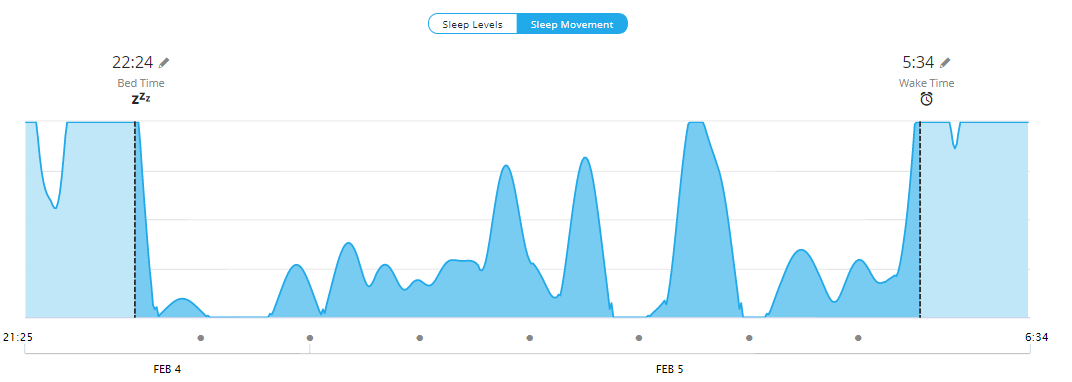
\includegraphics{images/sleep_data_graph.PNG}

My Garmin Vivosmart watch tracks the time I fall asleep and wake up each
day using motion sensing and heart rate monitoring. To augment this
data, I have estimated likelihoods that I am asleep based on the
condition of my bedroom light (on/off) and if my phone is charging
(yes/no). My objective is to use this data to create a model that
returns the probability I am asleep at a specific time for a given
status of my bedroom light and phone. For a specific time, the
probability of sleep given information about my bedroom light and phone
is expressed as:

\[P(\text{sleep} | \text{bedroom light}, \text{phone charging})\].

In probability theory terms, this is the posterior probability at a
specific time I am asleep given the status of my bedroom light and
condition of my phone. The time is a continuous variable and the two
additional pieces of information are discrete variables each with two
states.

    \hypertarget{approach}{%
\subsection{Approach}\label{approach}}

In order to solve this problem, I first need to express the final model
in terms of Bayes Rule. At a specific time, the probability of sleep
given my light and phone is:

\[P(s|L, C) = \frac{P(L, C|s) * P (s)}{P(L, C)}\]

Where \(P(s)\) is the sleep probability \(t\) is the time, \(L\) is the
condition of my bedroom light (on/off), and \(C\) is the charging status
of my phone (yes/no).

\(P(s)\) is the prior probability of sleep at the specified time. As
time is a continuous varible, we will use an approximate Markov Chain
Monte Carlo method to find the \emph{most likely} probability
distribution to find the prior.

One main assumption we make to simplify the inference is that the
probability of my bedroom light condition and phone charging status are
independent of one another with the knowledge of whether or not I am
asleep. That is, these discrete variables are conditionally independent
on sleep. Applying this assumption, the final model becomes at a
specific time becomes:

\[P(s | L, C) = \frac{(P(L|s) * P(C|s) * P(s)}{P(L|s) * P(C|s) * P(s) + P(L|\bar{s}) * P(C|\bar{s}) * P(\bar{s})}\]

This is the final expanded expression we need to solve to find the
posterior probability I am asleep at a specific time given the knowledge
of my bedroom light and phone charging.

Time is a continuous variable, and specifying the entire joint
probability for sleep given the time, \(P(s)\) would be infeasible even
with time discretized into one-minute intervals. Therefore, we will use
an approximate method, Markov Chain Monte Carlo (MCMC), to find the
posterior probability parameters. Markov Chain Monte Carlo samples based
on maximizing the likelihood of the parameters under the data. To find
the most likely posterior probability distribution of sleep given the
time, we can use the average of all the samples of the parameters.

After the posterior probability of sleep as a function of time,
\(P(s)\), has been calculated, this becomes the prior in the final
model. The other two variables, \(C\) and \(L\), are discrete, which
means we can specify the entire joint probability rather easily. The
final model uses Bayes Rule to update the probability of sleep with the
additional information. This represents the essence of Bayesian
inference: attempting to become less wrong by updating predictions based
on new evidence.

The general method is as follows, with additional details provided in
the respective sections.

\begin{enumerate}
\def\labelenumi{\arabic{enumi}.}
\tightlist
\item
  Format the data (done in separate notebook) and visualize
\item
  Choose function to represent probabilty of sleep given the time
\item
  Use Markov Chain Monte Carlo and the data to find most likely
  parameters for the selected posterior distribution
\item
  Use the posterior probability as the prior for applying Bayes Rule
  using additional data about light and phone status
\item
  Build a model for Bayesian Inference to find the probabilty of sleep
  given the time, light condition, and phone charging info
\item
  Interpret and visualize model
\end{enumerate}

We can do this separately for both the sleep and waking data, although I
will only build the complete model for the sleep data.

I make extensive use of the
\href{https://github.com/pymc-devs/pymc3}{PyMC3 library} for Markov
Chain Monte Carlo and Bayesian Inference methods in this report.

    \hypertarget{wake-and-sleep-data-exploration}{%
\section{Wake and Sleep Data
Exploration}\label{wake-and-sleep-data-exploration}}

The wake and sleep data contains more than two months of information.
The Garmin watch records when I fall asleep and wake up based on motion
and heart rate. It is not 100\% accurate as it often will think I'm
sleeping if I turn off notifications and am quietly reading in bed.
Sometimes we have to deal with imperfect data, and, because there are
more truthful than false observations, we can expect the correct data to
have a larger effect on the model.

First, we will import the required libraries, and visualize both the
sleep data and the waking data.

    \begin{Verbatim}[commandchars=\\\{\}]
{\color{incolor}In [{\color{incolor}1}]:} \PY{c+c1}{\PYZsh{} pandas and numpy for data manipulation}
        \PY{k+kn}{import} \PY{n+nn}{pandas} \PY{k}{as} \PY{n+nn}{pd}
        \PY{k+kn}{import} \PY{n+nn}{numpy} \PY{k}{as} \PY{n+nn}{np}
        
        \PY{c+c1}{\PYZsh{} scipy for algorithms}
        \PY{k+kn}{import} \PY{n+nn}{scipy}
        \PY{k+kn}{from} \PY{n+nn}{scipy} \PY{k}{import} \PY{n}{stats}
        
        \PY{c+c1}{\PYZsh{} pymc3 for Bayesian Inference, pymc built on t}
        \PY{k+kn}{import} \PY{n+nn}{pymc3} \PY{k}{as} \PY{n+nn}{pm}
        \PY{k+kn}{import} \PY{n+nn}{theano}\PY{n+nn}{.}\PY{n+nn}{tensor} \PY{k}{as} \PY{n+nn}{tt}
        \PY{k+kn}{import} \PY{n+nn}{scipy}
        
        \PY{c+c1}{\PYZsh{} matplotlib for plotting}
        \PY{k+kn}{import} \PY{n+nn}{matplotlib}\PY{n+nn}{.}\PY{n+nn}{pyplot} \PY{k}{as} \PY{n+nn}{plt}
        \PY{o}{\PYZpc{}}\PY{k}{matplotlib} inline
        \PY{k+kn}{from} \PY{n+nn}{IPython}\PY{n+nn}{.}\PY{n+nn}{core}\PY{n+nn}{.}\PY{n+nn}{pylabtools} \PY{k}{import} \PY{n}{figsize}
        \PY{k+kn}{import} \PY{n+nn}{matplotlib}
        
        \PY{k+kn}{import} \PY{n+nn}{json}
        \PY{n}{s} \PY{o}{=} \PY{n}{json}\PY{o}{.}\PY{n}{load}\PY{p}{(}\PY{n+nb}{open}\PY{p}{(}\PY{l+s+s1}{\PYZsq{}}\PY{l+s+s1}{style/bmh\PYZus{}matplotlibrc.json}\PY{l+s+s1}{\PYZsq{}}\PY{p}{)}\PY{p}{)}
        \PY{n}{matplotlib}\PY{o}{.}\PY{n}{rcParams}\PY{o}{.}\PY{n}{update}\PY{p}{(}\PY{n}{s}\PY{p}{)}
        \PY{n}{matplotlib}\PY{o}{.}\PY{n}{rcParams}\PY{p}{[}\PY{l+s+s1}{\PYZsq{}}\PY{l+s+s1}{figure.figsize}\PY{l+s+s1}{\PYZsq{}}\PY{p}{]} \PY{o}{=} \PY{p}{(}\PY{l+m+mi}{10}\PY{p}{,} \PY{l+m+mi}{3}\PY{p}{)}
        \PY{n}{matplotlib}\PY{o}{.}\PY{n}{rcParams}\PY{p}{[}\PY{l+s+s1}{\PYZsq{}}\PY{l+s+s1}{font.size}\PY{l+s+s1}{\PYZsq{}}\PY{p}{]} \PY{o}{=} \PY{l+m+mi}{14}
        
        \PY{c+c1}{\PYZsh{} Number of samples for Markov Chain Monte Carlo}
        \PY{n}{N\PYZus{}SAMPLES} \PY{o}{=} \PY{l+m+mi}{5000}
\end{Verbatim}


    \begin{Verbatim}[commandchars=\\\{\}]
WARNING (theano.tensor.blas): Using NumPy C-API based implementation for BLAS functions.

    \end{Verbatim}

    \begin{Verbatim}[commandchars=\\\{\}]
{\color{incolor}In [{\color{incolor}2}]:} \PY{c+c1}{\PYZsh{} Data formatted in different notebook}
        \PY{n}{sleep\PYZus{}data} \PY{o}{=} \PY{n}{pd}\PY{o}{.}\PY{n}{read\PYZus{}csv}\PY{p}{(}\PY{l+s+s1}{\PYZsq{}}\PY{l+s+s1}{data/sleep\PYZus{}data.csv}\PY{l+s+s1}{\PYZsq{}}\PY{p}{)}
        \PY{n}{wake\PYZus{}data} \PY{o}{=} \PY{n}{pd}\PY{o}{.}\PY{n}{read\PYZus{}csv}\PY{p}{(}\PY{l+s+s1}{\PYZsq{}}\PY{l+s+s1}{data/wake\PYZus{}data.csv}\PY{l+s+s1}{\PYZsq{}}\PY{p}{)}
        
        \PY{c+c1}{\PYZsh{} Labels for plotting}
        \PY{n}{sleep\PYZus{}labels} \PY{o}{=} \PY{p}{[}\PY{l+s+s1}{\PYZsq{}}\PY{l+s+s1}{9:00}\PY{l+s+s1}{\PYZsq{}}\PY{p}{,} \PY{l+s+s1}{\PYZsq{}}\PY{l+s+s1}{9:30}\PY{l+s+s1}{\PYZsq{}}\PY{p}{,} \PY{l+s+s1}{\PYZsq{}}\PY{l+s+s1}{10:00}\PY{l+s+s1}{\PYZsq{}}\PY{p}{,} \PY{l+s+s1}{\PYZsq{}}\PY{l+s+s1}{10:30}\PY{l+s+s1}{\PYZsq{}}\PY{p}{,} \PY{l+s+s1}{\PYZsq{}}\PY{l+s+s1}{11:00}\PY{l+s+s1}{\PYZsq{}}\PY{p}{,} \PY{l+s+s1}{\PYZsq{}}\PY{l+s+s1}{11:30}\PY{l+s+s1}{\PYZsq{}}\PY{p}{,} \PY{l+s+s1}{\PYZsq{}}\PY{l+s+s1}{12:00}\PY{l+s+s1}{\PYZsq{}}\PY{p}{]}
        \PY{n}{wake\PYZus{}labels} \PY{o}{=} \PY{p}{[}\PY{l+s+s1}{\PYZsq{}}\PY{l+s+s1}{5:00}\PY{l+s+s1}{\PYZsq{}}\PY{p}{,} \PY{l+s+s1}{\PYZsq{}}\PY{l+s+s1}{5:30}\PY{l+s+s1}{\PYZsq{}}\PY{p}{,} \PY{l+s+s1}{\PYZsq{}}\PY{l+s+s1}{6:00}\PY{l+s+s1}{\PYZsq{}}\PY{p}{,} \PY{l+s+s1}{\PYZsq{}}\PY{l+s+s1}{6:30}\PY{l+s+s1}{\PYZsq{}}\PY{p}{,} \PY{l+s+s1}{\PYZsq{}}\PY{l+s+s1}{7:00}\PY{l+s+s1}{\PYZsq{}}\PY{p}{,} \PY{l+s+s1}{\PYZsq{}}\PY{l+s+s1}{7:30}\PY{l+s+s1}{\PYZsq{}}\PY{p}{,} \PY{l+s+s1}{\PYZsq{}}\PY{l+s+s1}{8:00}\PY{l+s+s1}{\PYZsq{}}\PY{p}{]}
\end{Verbatim}


    \hypertarget{falling-asleep-data}{%
\subsection{Falling Asleep Data}\label{falling-asleep-data}}

Each dot represents one observation at a specific time with the color
intensity corresponding to the number of points at that time. We can see
that I tend to fall asleep a little after 10:00 PM.

    \begin{Verbatim}[commandchars=\\\{\}]
{\color{incolor}In [{\color{incolor}3}]:} \PY{n}{figsize}\PY{p}{(}\PY{l+m+mi}{16}\PY{p}{,} \PY{l+m+mi}{4}\PY{p}{)}
        
        \PY{c+c1}{\PYZsh{} Sleep data}
        \PY{n}{plt}\PY{o}{.}\PY{n}{scatter}\PY{p}{(}\PY{n}{sleep\PYZus{}data}\PY{p}{[}\PY{l+s+s1}{\PYZsq{}}\PY{l+s+s1}{time\PYZus{}offset}\PY{l+s+s1}{\PYZsq{}}\PY{p}{]}\PY{p}{,} \PY{n}{sleep\PYZus{}data}\PY{p}{[}\PY{l+s+s1}{\PYZsq{}}\PY{l+s+s1}{indicator}\PY{l+s+s1}{\PYZsq{}}\PY{p}{]}\PY{p}{,} 
                    \PY{n}{s}\PY{o}{=} \PY{l+m+mi}{60}\PY{p}{,} \PY{n}{alpha}\PY{o}{=}\PY{l+m+mf}{0.01}\PY{p}{,} \PY{n}{facecolor} \PY{o}{=} \PY{l+s+s1}{\PYZsq{}}\PY{l+s+s1}{b}\PY{l+s+s1}{\PYZsq{}}\PY{p}{,} \PY{n}{edgecolors}\PY{o}{=}\PY{l+s+s1}{\PYZsq{}}\PY{l+s+s1}{b}\PY{l+s+s1}{\PYZsq{}}\PY{p}{)}
        \PY{n}{plt}\PY{o}{.}\PY{n}{yticks}\PY{p}{(}\PY{p}{[}\PY{l+m+mi}{0}\PY{p}{,} \PY{l+m+mi}{1}\PY{p}{]}\PY{p}{,} \PY{p}{[}\PY{l+s+s1}{\PYZsq{}}\PY{l+s+s1}{Awake}\PY{l+s+s1}{\PYZsq{}}\PY{p}{,} \PY{l+s+s1}{\PYZsq{}}\PY{l+s+s1}{Asleep}\PY{l+s+s1}{\PYZsq{}}\PY{p}{]}\PY{p}{)}\PY{p}{;} \PY{n}{plt}\PY{o}{.}\PY{n}{xlabel}\PY{p}{(}\PY{l+s+s1}{\PYZsq{}}\PY{l+s+s1}{PM Time}\PY{l+s+s1}{\PYZsq{}}\PY{p}{)}\PY{p}{;} 
        \PY{n}{plt}\PY{o}{.}\PY{n}{title}\PY{p}{(}\PY{l+s+s1}{\PYZsq{}}\PY{l+s+s1}{Falling Asleep Data}\PY{l+s+s1}{\PYZsq{}}\PY{p}{)}
        \PY{n}{plt}\PY{o}{.}\PY{n}{xticks}\PY{p}{(}\PY{p}{[}\PY{o}{\PYZhy{}}\PY{l+m+mi}{60}\PY{p}{,} \PY{o}{\PYZhy{}}\PY{l+m+mi}{30}\PY{p}{,} \PY{l+m+mi}{0}\PY{p}{,} \PY{l+m+mi}{30}\PY{p}{,} \PY{l+m+mi}{60}\PY{p}{,} \PY{l+m+mi}{90}\PY{p}{,} \PY{l+m+mi}{120}\PY{p}{]}\PY{p}{,} \PY{n}{sleep\PYZus{}labels}\PY{p}{)}\PY{p}{;}
\end{Verbatim}


    \begin{center}
    \adjustimage{max size={0.9\linewidth}{0.9\paperheight}}{assign_1_files/assign_1_6_0.png}
    \end{center}
    { \hspace*{\fill} \\}
    
    \hypertarget{waking-up-data}{%
\subsection{Waking Up Data}\label{waking-up-data}}

My alarm is set for 6:00 AM every day of the week, and the wake data is
more consistent than the sleep data. I nearly always wake up within a 10
minute window around 6:00 AM.

    \begin{Verbatim}[commandchars=\\\{\}]
{\color{incolor}In [{\color{incolor}4}]:} \PY{c+c1}{\PYZsh{} Wake data}
        \PY{n}{plt}\PY{o}{.}\PY{n}{scatter}\PY{p}{(}\PY{n}{wake\PYZus{}data}\PY{p}{[}\PY{l+s+s1}{\PYZsq{}}\PY{l+s+s1}{time\PYZus{}offset}\PY{l+s+s1}{\PYZsq{}}\PY{p}{]}\PY{p}{,} \PY{n}{wake\PYZus{}data}\PY{p}{[}\PY{l+s+s1}{\PYZsq{}}\PY{l+s+s1}{indicator}\PY{l+s+s1}{\PYZsq{}}\PY{p}{]}\PY{p}{,} 
                    \PY{n}{s}\PY{o}{=} \PY{l+m+mi}{50}\PY{p}{,} \PY{n}{alpha} \PY{o}{=} \PY{l+m+mf}{0.01}\PY{p}{,} \PY{n}{facecolor}\PY{o}{=}\PY{l+s+s1}{\PYZsq{}}\PY{l+s+s1}{r}\PY{l+s+s1}{\PYZsq{}}\PY{p}{,} \PY{n}{edgecolors} \PY{o}{=}  \PY{l+s+s1}{\PYZsq{}}\PY{l+s+s1}{r}\PY{l+s+s1}{\PYZsq{}}\PY{p}{)}\PY{p}{;}
        \PY{n}{plt}\PY{o}{.}\PY{n}{yticks}\PY{p}{(}\PY{p}{[}\PY{l+m+mi}{0}\PY{p}{,} \PY{l+m+mi}{1}\PY{p}{]}\PY{p}{,} \PY{p}{[}\PY{l+s+s1}{\PYZsq{}}\PY{l+s+s1}{Awake}\PY{l+s+s1}{\PYZsq{}}\PY{p}{,} \PY{l+s+s1}{\PYZsq{}}\PY{l+s+s1}{Asleep}\PY{l+s+s1}{\PYZsq{}}\PY{p}{]}\PY{p}{)}\PY{p}{;} \PY{n}{plt}\PY{o}{.}\PY{n}{xlabel}\PY{p}{(}\PY{l+s+s1}{\PYZsq{}}\PY{l+s+s1}{AM Time}\PY{l+s+s1}{\PYZsq{}}\PY{p}{)}\PY{p}{;}
        \PY{n}{plt}\PY{o}{.}\PY{n}{title}\PY{p}{(}\PY{l+s+s1}{\PYZsq{}}\PY{l+s+s1}{Waking Up Data}\PY{l+s+s1}{\PYZsq{}}\PY{p}{)}
        \PY{n}{plt}\PY{o}{.}\PY{n}{xticks}\PY{p}{(}\PY{p}{[}\PY{o}{\PYZhy{}}\PY{l+m+mi}{60}\PY{p}{,} \PY{o}{\PYZhy{}}\PY{l+m+mi}{30}\PY{p}{,} \PY{l+m+mi}{0}\PY{p}{,} \PY{l+m+mi}{30}\PY{p}{,} \PY{l+m+mi}{60}\PY{p}{,} \PY{l+m+mi}{90}\PY{p}{,} \PY{l+m+mi}{120}\PY{p}{]}\PY{p}{,} \PY{n}{wake\PYZus{}labels}\PY{p}{)}\PY{p}{;}
\end{Verbatim}


    \begin{center}
    \adjustimage{max size={0.9\linewidth}{0.9\paperheight}}{assign_1_files/assign_1_8_0.png}
    \end{center}
    { \hspace*{\fill} \\}
    
    \hypertarget{logistic-function-to-represent-transition}{%
\section{Logistic Function to Represent
Transition}\label{logistic-function-to-represent-transition}}

We need to decide on a function to represent the transition from being
awake to sleeping. There are a number of acceptable models, and here we
will assume this transition can be modeled as a logistic function. A
logistic function (also called a sigmoid) is a non-linear function
bounded between 0 and 1. As \({t \to -\infty}, {p(s) \to 0}\) and, as
\({t \to +\infty}, {p(s) \to 1}\). The expression for a logistic
probability distribution for sleep as a function of time is:

\[p(s) = \frac{1}{ 1 + e^{\;\beta t } }\]

The \(\beta\) parameter is unknown and be esimated using Markov Chain
Monte Carlo sampling. MCMC samples from the prior for each parameter,
trying to maximize the probabilty of the parameter given the data.

Several logistic functions with various \(\beta\) parameters are shown
below:

    \begin{Verbatim}[commandchars=\\\{\}]
{\color{incolor}In [{\color{incolor}5}]:} \PY{n}{figsize}\PY{p}{(}\PY{l+m+mi}{16}\PY{p}{,} \PY{l+m+mi}{6}\PY{p}{)}
        
        \PY{c+c1}{\PYZsh{} Logistic function with only beta}
        \PY{k}{def} \PY{n+nf}{logistic}\PY{p}{(}\PY{n}{x}\PY{p}{,} \PY{n}{beta}\PY{p}{)}\PY{p}{:}
            \PY{k}{return} \PY{l+m+mf}{1.} \PY{o}{/} \PY{p}{(}\PY{l+m+mf}{1.} \PY{o}{+} \PY{n}{np}\PY{o}{.}\PY{n}{exp}\PY{p}{(}\PY{n}{beta} \PY{o}{*} \PY{n}{x}\PY{p}{)}\PY{p}{)}
        
        \PY{c+c1}{\PYZsh{} Plot examples with different betas }
        \PY{n}{x} \PY{o}{=} \PY{n}{np}\PY{o}{.}\PY{n}{linspace}\PY{p}{(}\PY{o}{\PYZhy{}}\PY{l+m+mi}{5}\PY{p}{,} \PY{l+m+mi}{5}\PY{p}{,} \PY{l+m+mi}{1000}\PY{p}{)}
        \PY{k}{for} \PY{n}{beta} \PY{o+ow}{in} \PY{p}{[}\PY{o}{\PYZhy{}}\PY{l+m+mi}{5}\PY{p}{,} \PY{o}{\PYZhy{}}\PY{l+m+mi}{1}\PY{p}{,} \PY{l+m+mf}{0.5}\PY{p}{,} \PY{l+m+mi}{1}\PY{p}{,} \PY{l+m+mi}{5}\PY{p}{]}\PY{p}{:}
            \PY{n}{plt}\PY{o}{.}\PY{n}{plot}\PY{p}{(}\PY{n}{x}\PY{p}{,} \PY{n}{logistic}\PY{p}{(}\PY{n}{x}\PY{p}{,} \PY{n}{beta}\PY{p}{)}\PY{p}{,} \PY{n}{label} \PY{o}{=} \PY{l+s+sa}{r}\PY{l+s+s2}{\PYZdq{}}\PY{l+s+s2}{\PYZdl{}}\PY{l+s+s2}{\PYZbs{}}\PY{l+s+s2}{beta\PYZdl{} = }\PY{l+s+si}{\PYZpc{}.1f}\PY{l+s+s2}{\PYZdq{}} \PY{o}{\PYZpc{}} \PY{n}{beta}\PY{p}{)}
        
        \PY{n}{plt}\PY{o}{.}\PY{n}{legend}\PY{p}{(}\PY{p}{)}\PY{p}{;}
        \PY{n}{plt}\PY{o}{.}\PY{n}{title}\PY{p}{(}\PY{l+s+sa}{r}\PY{l+s+s1}{\PYZsq{}}\PY{l+s+s1}{Logistic Function with Different \PYZdl{}}\PY{l+s+s1}{\PYZbs{}}\PY{l+s+s1}{beta\PYZdl{} values}\PY{l+s+s1}{\PYZsq{}}\PY{p}{)}\PY{p}{;}
\end{Verbatim}


    \begin{center}
    \adjustimage{max size={0.9\linewidth}{0.9\paperheight}}{assign_1_files/assign_1_10_0.png}
    \end{center}
    { \hspace*{\fill} \\}
    
    There is one problem with the basic logistic function as shown above:
the transition is centered at 0. However, in my sleeping data, the
transition is around 10:00 pm for sleeping and 6:00 am for waking. We
address this by adding an offset, called a bias, to adjust the location
of the logistic function. The logistic function now is:

\[P(s) = \frac{1}{ 1 + e^{\;\beta t + \alpha} }\]

This introduces another unknown parameter, \(\alpha\), which we will
also find from Markov Chain Monte Carlo.

The logistic function with various \(\alpha\) and \(\beta\) parameters
is shown below.

    \begin{Verbatim}[commandchars=\\\{\}]
{\color{incolor}In [{\color{incolor}6}]:} \PY{c+c1}{\PYZsh{} Logistic function with both beta and alpha}
        \PY{k}{def} \PY{n+nf}{logistic}\PY{p}{(}\PY{n}{x}\PY{p}{,} \PY{n}{beta}\PY{p}{,} \PY{n}{alpha}\PY{o}{=}\PY{l+m+mi}{0}\PY{p}{)}\PY{p}{:}
            \PY{k}{return} \PY{l+m+mf}{1.0} \PY{o}{/} \PY{p}{(}\PY{l+m+mf}{1.0} \PY{o}{+} \PY{n}{np}\PY{o}{.}\PY{n}{exp}\PY{p}{(}\PY{n}{np}\PY{o}{.}\PY{n}{dot}\PY{p}{(}\PY{n}{beta}\PY{p}{,} \PY{n}{x}\PY{p}{)} \PY{o}{+} \PY{n}{alpha}\PY{p}{)}\PY{p}{)}
        
        \PY{n}{x} \PY{o}{=} \PY{n}{np}\PY{o}{.}\PY{n}{linspace}\PY{p}{(}\PY{o}{\PYZhy{}}\PY{l+m+mi}{5}\PY{p}{,} \PY{l+m+mi}{5}\PY{p}{,} \PY{l+m+mi}{1000}\PY{p}{)}
        
        \PY{n}{plt}\PY{o}{.}\PY{n}{plot}\PY{p}{(}\PY{n}{x}\PY{p}{,} \PY{n}{logistic}\PY{p}{(}\PY{n}{x}\PY{p}{,} \PY{n}{beta}\PY{o}{=}\PY{l+m+mi}{1}\PY{p}{)}\PY{p}{,} \PY{n}{label}\PY{o}{=}\PY{l+s+sa}{r}\PY{l+s+s2}{\PYZdq{}}\PY{l+s+s2}{\PYZdl{}}\PY{l+s+s2}{\PYZbs{}}\PY{l+s+s2}{beta = 1\PYZdl{}}\PY{l+s+s2}{\PYZdq{}}\PY{p}{,} \PY{n}{ls}\PY{o}{=}\PY{l+s+s2}{\PYZdq{}}\PY{l+s+s2}{\PYZhy{}\PYZhy{}}\PY{l+s+s2}{\PYZdq{}}\PY{p}{,} \PY{n}{lw}\PY{o}{=}\PY{l+m+mi}{2}\PY{p}{)}
        \PY{n}{plt}\PY{o}{.}\PY{n}{plot}\PY{p}{(}\PY{n}{x}\PY{p}{,} \PY{n}{logistic}\PY{p}{(}\PY{n}{x}\PY{p}{,} \PY{n}{beta}\PY{o}{=}\PY{o}{\PYZhy{}}\PY{l+m+mi}{1}\PY{p}{)}\PY{p}{,} \PY{n}{label}\PY{o}{=}\PY{l+s+sa}{r}\PY{l+s+s2}{\PYZdq{}}\PY{l+s+s2}{\PYZdl{}}\PY{l+s+s2}{\PYZbs{}}\PY{l+s+s2}{beta = \PYZhy{}1\PYZdl{}}\PY{l+s+s2}{\PYZdq{}}\PY{p}{,} \PY{n}{ls}\PY{o}{=}\PY{l+s+s2}{\PYZdq{}}\PY{l+s+s2}{\PYZhy{}\PYZhy{}}\PY{l+s+s2}{\PYZdq{}}\PY{p}{,} \PY{n}{lw}\PY{o}{=}\PY{l+m+mi}{2}\PY{p}{)}
        
        \PY{n}{plt}\PY{o}{.}\PY{n}{plot}\PY{p}{(}\PY{n}{x}\PY{p}{,} \PY{n}{logistic}\PY{p}{(}\PY{n}{x}\PY{p}{,} \PY{l+m+mi}{1}\PY{p}{,} \PY{l+m+mi}{1}\PY{p}{)}\PY{p}{,} 
                 \PY{n}{label}\PY{o}{=}\PY{l+s+sa}{r}\PY{l+s+s2}{\PYZdq{}}\PY{l+s+s2}{\PYZdl{}}\PY{l+s+s2}{\PYZbs{}}\PY{l+s+s2}{beta = 1, }\PY{l+s+s2}{\PYZbs{}}\PY{l+s+s2}{alpha = 1\PYZdl{}}\PY{l+s+s2}{\PYZdq{}}\PY{p}{,} \PY{n}{color}\PY{o}{=}\PY{l+s+s2}{\PYZdq{}}\PY{l+s+s2}{darkblue}\PY{l+s+s2}{\PYZdq{}}\PY{p}{)}
        \PY{n}{plt}\PY{o}{.}\PY{n}{plot}\PY{p}{(}\PY{n}{x}\PY{p}{,} \PY{n}{logistic}\PY{p}{(}\PY{n}{x}\PY{p}{,} \PY{l+m+mi}{1}\PY{p}{,} \PY{o}{\PYZhy{}}\PY{l+m+mi}{1}\PY{p}{)}\PY{p}{,}
                 \PY{n}{label}\PY{o}{=}\PY{l+s+sa}{r}\PY{l+s+s2}{\PYZdq{}}\PY{l+s+s2}{\PYZdl{}}\PY{l+s+s2}{\PYZbs{}}\PY{l+s+s2}{beta = 1, }\PY{l+s+s2}{\PYZbs{}}\PY{l+s+s2}{alpha = \PYZhy{}1\PYZdl{}}\PY{l+s+s2}{\PYZdq{}}\PY{p}{,}\PY{n}{color}\PY{o}{=}\PY{l+s+s2}{\PYZdq{}}\PY{l+s+s2}{skyblue}\PY{l+s+s2}{\PYZdq{}}\PY{p}{)}
        \PY{n}{plt}\PY{o}{.}\PY{n}{plot}\PY{p}{(}\PY{n}{x}\PY{p}{,} \PY{n}{logistic}\PY{p}{(}\PY{n}{x}\PY{p}{,} \PY{o}{\PYZhy{}}\PY{l+m+mi}{1}\PY{p}{,} \PY{l+m+mi}{5}\PY{p}{)}\PY{p}{,} 
                 \PY{n}{label}\PY{o}{=}\PY{l+s+sa}{r}\PY{l+s+s2}{\PYZdq{}}\PY{l+s+s2}{\PYZdl{}}\PY{l+s+s2}{\PYZbs{}}\PY{l+s+s2}{beta = \PYZhy{}1, }\PY{l+s+s2}{\PYZbs{}}\PY{l+s+s2}{alpha = 5\PYZdl{}}\PY{l+s+s2}{\PYZdq{}}\PY{p}{,} \PY{n}{color}\PY{o}{=}\PY{l+s+s2}{\PYZdq{}}\PY{l+s+s2}{orangered}\PY{l+s+s2}{\PYZdq{}}\PY{p}{)}
        \PY{n}{plt}\PY{o}{.}\PY{n}{plot}\PY{p}{(}\PY{n}{x}\PY{p}{,} \PY{n}{logistic}\PY{p}{(}\PY{n}{x}\PY{p}{,} \PY{o}{\PYZhy{}}\PY{l+m+mi}{1}\PY{p}{,} \PY{o}{\PYZhy{}}\PY{l+m+mi}{5}\PY{p}{)}\PY{p}{,} 
                 \PY{n}{label}\PY{o}{=}\PY{l+s+sa}{r}\PY{l+s+s2}{\PYZdq{}}\PY{l+s+s2}{\PYZdl{}}\PY{l+s+s2}{\PYZbs{}}\PY{l+s+s2}{beta = \PYZhy{}1, }\PY{l+s+s2}{\PYZbs{}}\PY{l+s+s2}{alpha = \PYZhy{}5\PYZdl{}}\PY{l+s+s2}{\PYZdq{}}\PY{p}{,} \PY{n}{color}\PY{o}{=}\PY{l+s+s2}{\PYZdq{}}\PY{l+s+s2}{darkred}\PY{l+s+s2}{\PYZdq{}}\PY{p}{)}
        \PY{n}{plt}\PY{o}{.}\PY{n}{legend}\PY{p}{(}\PY{p}{)}\PY{p}{;}
        \PY{n}{plt}\PY{o}{.}\PY{n}{title}\PY{p}{(}\PY{l+s+sa}{r}\PY{l+s+s1}{\PYZsq{}}\PY{l+s+s1}{Logistic Function with Varying \PYZdl{}}\PY{l+s+s1}{\PYZbs{}}\PY{l+s+s1}{beta\PYZdl{} and \PYZdl{}}\PY{l+s+s1}{\PYZbs{}}\PY{l+s+s1}{alpha\PYZdl{}}\PY{l+s+s1}{\PYZsq{}}\PY{p}{)}\PY{p}{;}
\end{Verbatim}


    \begin{center}
    \adjustimage{max size={0.9\linewidth}{0.9\paperheight}}{assign_1_files/assign_1_12_0.png}
    \end{center}
    { \hspace*{\fill} \\}
    
    \(\beta\) shifts the direction and steepness of the curve, while
\(\alpha\) changes the location. We will use MCMC to find the most
likely value of these parameters under the data.

    \hypertarget{prior-distribution-for-beta-and-alpha}{%
\section{\texorpdfstring{Prior Distribution for \(\beta\) and
\(\alpha\)}{Prior Distribution for \textbackslash{}beta and \textbackslash{}alpha}}\label{prior-distribution-for-beta-and-alpha}}

We have no evidence to suggest what the prior distributions for the
model parameters \(\beta\) and \(\alpha\) are ahead of time. Therefore,
we can model them as if they came from a normal distribution. The
normal, or Gaussian, distribution is defined by the mean, \(\mu\), and
the precision, \(\tau\). The precision is the reciprocal of the standard
deviation, \(\sigma\). The mean defines the location of the distribution
and the precision shows the spread. A larger value of \(\tau\) indicates
the data is less spread out (it is more precise) and hence the variation
is smaller. The mean can be either positive or negative, but the
precision will always be positive. A normal distribution as defined here
is represented as:

\[ f(x | \mu, \tau) = \sqrt{\frac{\tau}{2\pi}} \exp\left( -\frac{\tau}{2} (x - \mu)^2 \right) \]

Probability density functions for three normal distributions are shown
below.

    \begin{Verbatim}[commandchars=\\\{\}]
{\color{incolor}In [{\color{incolor}7}]:} \PY{c+c1}{\PYZsh{} Set up the plotting parameters}
        \PY{n}{nor} \PY{o}{=} \PY{n}{stats}\PY{o}{.}\PY{n}{norm} 
        \PY{n}{x}\PY{o}{=} \PY{n}{np}\PY{o}{.}\PY{n}{linspace}\PY{p}{(}\PY{o}{\PYZhy{}}\PY{l+m+mi}{10}\PY{p}{,} \PY{l+m+mi}{10}\PY{p}{,} \PY{l+m+mi}{1000}\PY{p}{)}
        \PY{n}{mu} \PY{o}{=} \PY{p}{(}\PY{o}{\PYZhy{}}\PY{l+m+mi}{5}\PY{p}{,} \PY{l+m+mi}{0}\PY{p}{,} \PY{l+m+mi}{4}\PY{p}{)}
        \PY{n}{tau} \PY{o}{=} \PY{p}{(}\PY{l+m+mf}{0.5}\PY{p}{,} \PY{l+m+mi}{1}\PY{p}{,} \PY{l+m+mf}{2.5}\PY{p}{)}
        \PY{n}{colors} \PY{o}{=} \PY{p}{(}\PY{l+s+s2}{\PYZdq{}}\PY{l+s+s2}{turquoise}\PY{l+s+s2}{\PYZdq{}}\PY{p}{,} \PY{l+s+s2}{\PYZdq{}}\PY{l+s+s2}{orchid}\PY{l+s+s2}{\PYZdq{}}\PY{p}{,} \PY{l+s+s2}{\PYZdq{}}\PY{l+s+s2}{darkred}\PY{l+s+s2}{\PYZdq{}}\PY{p}{)}
        
        \PY{c+c1}{\PYZsh{} Plot 3 pdfs for different normal distributions}
        \PY{n}{params} \PY{o}{=} \PY{n+nb}{zip}\PY{p}{(}\PY{n}{mu}\PY{p}{,} \PY{n}{tau}\PY{p}{,} \PY{n}{colors}\PY{p}{)}
        \PY{k}{for} \PY{n}{param} \PY{o+ow}{in} \PY{n}{params}\PY{p}{:}
            \PY{n}{y} \PY{o}{=} \PY{n}{nor}\PY{o}{.}\PY{n}{pdf}\PY{p}{(}\PY{n}{x}\PY{p}{,} \PY{n}{loc} \PY{o}{=} \PY{n}{param}\PY{p}{[}\PY{l+m+mi}{0}\PY{p}{]}\PY{p}{,} \PY{n}{scale} \PY{o}{=} \PY{l+m+mi}{1} \PY{o}{/} \PY{n}{param}\PY{p}{[}\PY{l+m+mi}{1}\PY{p}{]}\PY{p}{)}
            \PY{n}{plt}\PY{o}{.}\PY{n}{plot}\PY{p}{(}\PY{n}{x}\PY{p}{,} \PY{n}{y}\PY{p}{,} 
                     \PY{n}{label}\PY{o}{=}\PY{l+s+s2}{\PYZdq{}}\PY{l+s+s2}{\PYZdl{}}\PY{l+s+s2}{\PYZbs{}}\PY{l+s+s2}{mu = }\PY{l+s+si}{\PYZpc{}d}\PY{l+s+s2}{,}\PY{l+s+s2}{\PYZbs{}}\PY{l+s+s2}{;}\PY{l+s+se}{\PYZbs{}\PYZbs{}}\PY{l+s+s2}{tau = }\PY{l+s+si}{\PYZpc{}.1f}\PY{l+s+s2}{\PYZdl{}}\PY{l+s+s2}{\PYZdq{}} \PY{o}{\PYZpc{}} \PY{p}{(}\PY{n}{param}\PY{p}{[}\PY{l+m+mi}{0}\PY{p}{]}\PY{p}{,} \PY{n}{param}\PY{p}{[}\PY{l+m+mi}{1}\PY{p}{]}\PY{p}{)}\PY{p}{,} 
                     \PY{n}{color} \PY{o}{=} \PY{n}{param}\PY{p}{[}\PY{l+m+mi}{2}\PY{p}{]}\PY{p}{)}
            \PY{n}{plt}\PY{o}{.}\PY{n}{fill\PYZus{}between}\PY{p}{(}\PY{n}{x}\PY{p}{,} \PY{n}{y}\PY{p}{,} \PY{n}{color} \PY{o}{=} \PY{n}{param}\PY{p}{[}\PY{l+m+mi}{2}\PY{p}{]}\PY{p}{,} \PY{n}{alpha} \PY{o}{=} \PY{l+m+mf}{0.3}\PY{p}{)}
            
        \PY{n}{plt}\PY{o}{.}\PY{n}{legend}\PY{p}{(}\PY{p}{)}\PY{p}{;}
        \PY{n}{plt}\PY{o}{.}\PY{n}{xlabel}\PY{p}{(}\PY{l+s+s2}{\PYZdq{}}\PY{l+s+s2}{\PYZdl{}x\PYZdl{}}\PY{l+s+s2}{\PYZdq{}}\PY{p}{)}
        \PY{n}{plt}\PY{o}{.}\PY{n}{ylabel}\PY{p}{(}\PY{l+s+s2}{\PYZdq{}}\PY{l+s+s2}{Probability Density}\PY{l+s+s2}{\PYZdq{}}\PY{p}{)}
        \PY{n}{plt}\PY{o}{.}\PY{n}{title}\PY{p}{(}\PY{l+s+s2}{\PYZdq{}}\PY{l+s+s2}{Probability Density Functions for Normal Distributions}\PY{l+s+s2}{\PYZdq{}}\PY{p}{)}\PY{p}{;}
\end{Verbatim}


    \begin{center}
    \adjustimage{max size={0.9\linewidth}{0.9\paperheight}}{assign_1_files/assign_1_15_0.png}
    \end{center}
    { \hspace*{\fill} \\}
    
    The expected value of a normal distribution is the mean.
\[ E[ X | \mu, \tau] = \mu\]

The variance of a normal distribution is equal to:

\[ Var[ X | \mu, \tau) = \frac{1}{\tau}\]

Again, we have no assumptions about the value for either \(\mu\) or
\(\tau\) in the prior distributions for \(\alpha\) and \(\beta\). When
we initialize the model, we can use \(\mu = 0\) and a relatively large
variance such as \(\tau = 0.05\). Markov Chain Monte Carlo will samples
values of \(\mu\) and \(\tau\) that try to maximize the likelihood of
\(\alpha\) and \(\beta\) under the data.

    \hypertarget{markov-chain-monte-carlo}{%
\subsection{Markov Chain Monte Carlo}\label{markov-chain-monte-carlo}}

    Markov Chain Monte Carlo will sample both \(\beta\) and \(\alpha\) from
two normal distributions to find the parameters. Each iteration (state),
an estimate for both \(\beta\) and \(\alpha\) are drawn from the prior.
If the parameters increase the probabilty of the data, the state is
accepted, but if the parameters are not in agreement with the data, the
state is rejected. Monte Carlo refers to the sampling part of the
algorithm. Markov Chain means that the next state is only dependent on
the current state in a first order process (second order depends on the
current and 1 previous step, third order on the current and 2 previous
steps and so on). MCMC will return every sample of the parameters for
the number of specified steps. This is known as the model trace. To find
the most likely parameters, we can take the average of the samples in
the trace. MCMC does not given an exact answer, but rather tries to find
the maximum likelihood states under the data.

When modeling with MCMC up to 50\% of the initial steps, referred to as
the burn-in part of the trace, are discarded because the algorithm
returns more likely parameters as the number of samples increases. The
initial samples are less likely than the latter samples on average.
There are a number of methods to test for convergence of MCMC, including
visually inspecting the trace, and calculating the auto-correlation of
the trace (a lower auto-correlation is an indicator of convergence). We
will look at the trace in this example, but will not take rigorous steps
to address convergence. There are also a number of methods to choose a
smart starting value for the Markov Chain such as Maximum A Posterior
estimation. Choosing an intelligent initial value can speed up
convergence.

    \hypertarget{posterior-probability-of-sleep-given-time}{%
\section{Posterior Probability of Sleep given
Time}\label{posterior-probability-of-sleep-given-time}}

We have all the pieces for the poesterior probabilty and can now put
them together. The logistic function describes the transition from awake
to asleep, but we do not konw the parameters \(\beta\) and \(\alpha\).
The aim is to find the parameters of the logistic function which
maximize the likelihood of the observed data. The parameters are assumed
to come from a normal distribution defined by a mean, \(\mu\) and a
variance, \(\tau\). The MCMC algorithm will sample values of \(\mu\) and
\(\tau\) for both \(\alpha\) and \(\beta\) to try and maximize the
parameters of the logistic function given the data.

The data is connected to the parameters through a Bernoulli Variable.

\hypertarget{bernoulli-variable}{%
\subsection{Bernoulli Variable}\label{bernoulli-variable}}

A bernoulli variable is a discrete random variable that is either 0 or
1. In our example, we can model asleep or awake as a Bernoulli variable
where awake is 0 and asleep is 1. The Bernoulli variable for sleep
depends on the time, in a manner defined by the logistic function.

\[ \text{Sleep Probability, $S_i$} \sim \text{Ber}( \;p(t_i)\; ), \;\; i=1..N\]

\(p(t_i)\) is the logistic function with the independent variable time,
so this becomes:

\[ P(\text{sleep}) = \text{Ber}(\frac{1}{1 + e^{(\beta t_i + \alpha)}})\]

The goal of MCMC is to find the \(\alpha\) and \(\beta\) parameters
using the data and assuming normal priors.

    \hypertarget{pymc3-model}{%
\subsubsection{PyMC3 Model}\label{pymc3-model}}

We are using a powerful Bayesian Inference library in Python called
PyMC3. This library has features for running Markov Chain Monte Carlo
and other inference algorithms. This report does not detail PyMC3, but a
great book for getting started is \emph{Probabilistic Programming and
Bayesian Methods for Hackers} by Cameron Davidson-Pilon which is
available for free on
\href{https://github.com/CamDavidsonPilon/Probabilistic-Programming-and-Bayesian-Methods-for-Hackers}{GitHub}

The following code creates the model and performs MCMC, drawing
\texttt{N\_SAMPLES} number of samples for \(\beta\) and \(\alpha\). The
specific sampling algorithm is
\href{http://www.mit.edu/~ilkery/papers/MetropolisHastingsSampling.pdf}{Metropolic
Hastings}. We feed in the data and tell the model it is observations of
the Bernoulli variable. The model then tries to maximize the parameters
under the data.

    \begin{Verbatim}[commandchars=\\\{\}]
{\color{incolor}In [{\color{incolor}8}]:} \PY{c+c1}{\PYZsh{} Sort the values by time offset}
        \PY{n}{sleep\PYZus{}data}\PY{o}{.}\PY{n}{sort\PYZus{}values}\PY{p}{(}\PY{l+s+s1}{\PYZsq{}}\PY{l+s+s1}{time\PYZus{}offset}\PY{l+s+s1}{\PYZsq{}}\PY{p}{,} \PY{n}{inplace}\PY{o}{=}\PY{k+kc}{True}\PY{p}{)}
        
        \PY{c+c1}{\PYZsh{} Time is the time offset}
        \PY{n}{time} \PY{o}{=} \PY{n}{np}\PY{o}{.}\PY{n}{array}\PY{p}{(}\PY{n}{sleep\PYZus{}data}\PY{o}{.}\PY{n}{loc}\PY{p}{[}\PY{p}{:}\PY{p}{,} \PY{l+s+s1}{\PYZsq{}}\PY{l+s+s1}{time\PYZus{}offset}\PY{l+s+s1}{\PYZsq{}}\PY{p}{]}\PY{p}{)}
        
        \PY{c+c1}{\PYZsh{} Observations are the indicator}
        \PY{n}{sleep\PYZus{}obs} \PY{o}{=} \PY{n}{np}\PY{o}{.}\PY{n}{array}\PY{p}{(}\PY{n}{sleep\PYZus{}data}\PY{o}{.}\PY{n}{loc}\PY{p}{[}\PY{p}{:}\PY{p}{,} \PY{l+s+s1}{\PYZsq{}}\PY{l+s+s1}{indicator}\PY{l+s+s1}{\PYZsq{}}\PY{p}{]}\PY{p}{)}
\end{Verbatim}


    \begin{Verbatim}[commandchars=\\\{\}]
{\color{incolor}In [{\color{incolor}9}]:} \PY{k}{with} \PY{n}{pm}\PY{o}{.}\PY{n}{Model}\PY{p}{(}\PY{p}{)} \PY{k}{as} \PY{n}{sleep\PYZus{}model}\PY{p}{:}
            \PY{c+c1}{\PYZsh{} Create the alpha and beta parameters}
            \PY{n}{alpha} \PY{o}{=} \PY{n}{pm}\PY{o}{.}\PY{n}{Normal}\PY{p}{(}\PY{l+s+s1}{\PYZsq{}}\PY{l+s+s1}{alpha}\PY{l+s+s1}{\PYZsq{}}\PY{p}{,} \PY{n}{mu}\PY{o}{=}\PY{l+m+mf}{0.0}\PY{p}{,} \PY{n}{tau}\PY{o}{=}\PY{l+m+mf}{0.05}\PY{p}{,} \PY{n}{testval}\PY{o}{=}\PY{l+m+mf}{0.0}\PY{p}{)}
            \PY{n}{beta} \PY{o}{=} \PY{n}{pm}\PY{o}{.}\PY{n}{Normal}\PY{p}{(}\PY{l+s+s1}{\PYZsq{}}\PY{l+s+s1}{beta}\PY{l+s+s1}{\PYZsq{}}\PY{p}{,} \PY{n}{mu}\PY{o}{=}\PY{l+m+mf}{0.0}\PY{p}{,} \PY{n}{tau}\PY{o}{=}\PY{l+m+mf}{0.05}\PY{p}{,} \PY{n}{testval}\PY{o}{=}\PY{l+m+mf}{0.0}\PY{p}{)}
            
            \PY{c+c1}{\PYZsh{} Create the probability from the logistic function}
            \PY{n}{p} \PY{o}{=} \PY{n}{pm}\PY{o}{.}\PY{n}{Deterministic}\PY{p}{(}\PY{l+s+s1}{\PYZsq{}}\PY{l+s+s1}{p}\PY{l+s+s1}{\PYZsq{}}\PY{p}{,} \PY{l+m+mf}{1.} \PY{o}{/} \PY{p}{(}\PY{l+m+mf}{1.} \PY{o}{+} \PY{n}{tt}\PY{o}{.}\PY{n}{exp}\PY{p}{(}\PY{n}{beta} \PY{o}{*} \PY{n}{time} \PY{o}{+} \PY{n}{alpha}\PY{p}{)}\PY{p}{)}\PY{p}{)}
            
            \PY{c+c1}{\PYZsh{} Create the bernoulli parameter which uses the observed data}
            \PY{n}{observed} \PY{o}{=} \PY{n}{pm}\PY{o}{.}\PY{n}{Bernoulli}\PY{p}{(}\PY{l+s+s1}{\PYZsq{}}\PY{l+s+s1}{obs}\PY{l+s+s1}{\PYZsq{}}\PY{p}{,} \PY{n}{p}\PY{p}{,} \PY{n}{observed}\PY{o}{=}\PY{n}{sleep\PYZus{}obs}\PY{p}{)}
            
            \PY{c+c1}{\PYZsh{} Starting values are found through Maximum A Posterior estimation}
            \PY{c+c1}{\PYZsh{} start = pm.find\PYZus{}MAP()}
            
            \PY{c+c1}{\PYZsh{} Using Metropolis Hastings Sampling}
            \PY{n}{step} \PY{o}{=} \PY{n}{pm}\PY{o}{.}\PY{n}{Metropolis}\PY{p}{(}\PY{p}{)}
            
            \PY{c+c1}{\PYZsh{} Sample from the posterior using the sampling method}
            \PY{n}{sleep\PYZus{}trace} \PY{o}{=} \PY{n}{pm}\PY{o}{.}\PY{n}{sample}\PY{p}{(}\PY{n}{N\PYZus{}SAMPLES}\PY{p}{,} \PY{n}{step}\PY{o}{=}\PY{n}{step}\PY{p}{)}\PY{p}{;}
\end{Verbatim}


    \begin{Verbatim}[commandchars=\\\{\}]
Multiprocess sampling (2 chains in 2 jobs)
CompoundStep
>Metropolis: [beta]
>Metropolis: [alpha]
The number of effective samples is smaller than 10\% for some parameters.

    \end{Verbatim}

    The \texttt{trace} variable contains all of the samples drawn from the
posterior for \(\beta\) and \(\alpha\). We can graph these samples to
explore how they change over the course of sampling. The idea of MCMC is
that the samples get more likely given the data as the algorithm
continues. In other words, the MCMC algorithm converges on the most
likely values as the samples increase. We expect the latter values drawn
from the posterior to be more accurate than the earlier values. In
Markov Chain Monte Carlo, it is common practice to discard a portion of
the samples, usually about 50\%, which are known as the burn-in samples.
For this report I am not discarding any samples, but in a real
application, we would run the model for many more steps and discard the
initial samples.

    \hypertarget{visualize-posteriors-for-beta-and-alpha}{%
\subsection{\texorpdfstring{Visualize Posteriors for \(\beta\) and
\(\alpha\)}{Visualize Posteriors for \textbackslash{}beta and \textbackslash{}alpha}}\label{visualize-posteriors-for-beta-and-alpha}}

The values returned in the \texttt{trace} are all the samples drawn for
the parameters. We can visually inspect these values in histograms.

    \begin{Verbatim}[commandchars=\\\{\}]
{\color{incolor}In [{\color{incolor}10}]:} \PY{c+c1}{\PYZsh{} Extract the alpha and beta samples}
         \PY{c+c1}{\PYZsh{} Currently using all, including the burn\PYZhy{}in period}
         \PY{n}{alpha\PYZus{}samples} \PY{o}{=} \PY{n}{sleep\PYZus{}trace}\PY{p}{[}\PY{l+s+s2}{\PYZdq{}}\PY{l+s+s2}{alpha}\PY{l+s+s2}{\PYZdq{}}\PY{p}{]}\PY{p}{[}\PY{p}{:}\PY{p}{,} \PY{k+kc}{None}\PY{p}{]}
         \PY{n}{beta\PYZus{}samples} \PY{o}{=} \PY{n}{sleep\PYZus{}trace}\PY{p}{[}\PY{l+s+s2}{\PYZdq{}}\PY{l+s+s2}{beta}\PY{l+s+s2}{\PYZdq{}}\PY{p}{]}\PY{p}{[}\PY{p}{:}\PY{p}{,} \PY{k+kc}{None}\PY{p}{]}
\end{Verbatim}


    \begin{Verbatim}[commandchars=\\\{\}]
{\color{incolor}In [{\color{incolor}11}]:} \PY{n}{figsize}\PY{p}{(}\PY{l+m+mi}{16}\PY{p}{,} \PY{l+m+mi}{10}\PY{p}{)}
         
         \PY{n}{plt}\PY{o}{.}\PY{n}{subplot}\PY{p}{(}\PY{l+m+mi}{211}\PY{p}{)}
         \PY{n}{plt}\PY{o}{.}\PY{n}{title}\PY{p}{(}\PY{l+s+sa}{r}\PY{l+s+s2}{\PYZdq{}\PYZdq{}\PYZdq{}}\PY{l+s+s2}{Posterior Distribution of the Parameters }
         \PY{l+s+s2}{\PYZdl{}}\PY{l+s+s2}{\PYZbs{}}\PY{l+s+s2}{alpha, }\PY{l+s+s2}{\PYZbs{}}\PY{l+s+s2}{beta\PYZdl{} with }\PY{l+s+si}{\PYZpc{}d}\PY{l+s+s2}{ samples}\PY{l+s+s2}{\PYZdq{}\PYZdq{}\PYZdq{}} \PY{o}{\PYZpc{}} \PY{n}{N\PYZus{}SAMPLES}\PY{p}{)}
         
         \PY{n}{plt}\PY{o}{.}\PY{n}{hist}\PY{p}{(}\PY{n}{alpha\PYZus{}samples}\PY{p}{,} \PY{n}{histtype}\PY{o}{=}\PY{l+s+s1}{\PYZsq{}}\PY{l+s+s1}{stepfilled}\PY{l+s+s1}{\PYZsq{}}\PY{p}{,} 
                  \PY{n}{color} \PY{o}{=} \PY{l+s+s1}{\PYZsq{}}\PY{l+s+s1}{darkred}\PY{l+s+s1}{\PYZsq{}}\PY{p}{,} \PY{n}{bins}\PY{o}{=}\PY{l+m+mi}{30}\PY{p}{,} \PY{n}{alpha}\PY{o}{=}\PY{l+m+mf}{0.8}\PY{p}{,} 
                  \PY{n}{label}\PY{o}{=}\PY{l+s+sa}{r}\PY{l+s+s2}{\PYZdq{}}\PY{l+s+s2}{posterior of \PYZdl{}}\PY{l+s+s2}{\PYZbs{}}\PY{l+s+s2}{alpha\PYZdl{}}\PY{l+s+s2}{\PYZdq{}}\PY{p}{,} \PY{n}{normed}\PY{o}{=}\PY{k+kc}{True}\PY{p}{)}\PY{p}{;}
         \PY{n}{plt}\PY{o}{.}\PY{n}{legend}\PY{p}{(}\PY{p}{)}
         
         \PY{n}{plt}\PY{o}{.}\PY{n}{subplot}\PY{p}{(}\PY{l+m+mi}{212}\PY{p}{)}
         
         \PY{n}{plt}\PY{o}{.}\PY{n}{hist}\PY{p}{(}\PY{n}{beta\PYZus{}samples}\PY{p}{,} \PY{n}{histtype}\PY{o}{=}\PY{l+s+s1}{\PYZsq{}}\PY{l+s+s1}{stepfilled}\PY{l+s+s1}{\PYZsq{}}\PY{p}{,} 
                  \PY{n}{color} \PY{o}{=} \PY{l+s+s1}{\PYZsq{}}\PY{l+s+s1}{darkblue}\PY{l+s+s1}{\PYZsq{}}\PY{p}{,} \PY{n}{bins}\PY{o}{=}\PY{l+m+mi}{30}\PY{p}{,} \PY{n}{alpha}\PY{o}{=}\PY{l+m+mf}{0.8}\PY{p}{,} 
                  \PY{n}{label}\PY{o}{=}\PY{l+s+sa}{r}\PY{l+s+s2}{\PYZdq{}}\PY{l+s+s2}{posterior of \PYZdl{}}\PY{l+s+s2}{\PYZbs{}}\PY{l+s+s2}{beta\PYZdl{}}\PY{l+s+s2}{\PYZdq{}}\PY{p}{,} \PY{n}{normed}\PY{o}{=}\PY{k+kc}{True}\PY{p}{)}
         \PY{n}{plt}\PY{o}{.}\PY{n}{legend}\PY{p}{(}\PY{p}{)}\PY{p}{;}
\end{Verbatim}


    \begin{center}
    \adjustimage{max size={0.9\linewidth}{0.9\paperheight}}{assign_1_files/assign_1_26_0.png}
    \end{center}
    { \hspace*{\fill} \\}
    
    If the \(\beta\) values were centered around 0 that would indicate time
has no effect on the probability of being asleep. The \(\alpha\) values
also are not at 0, indicating that there is an offset from 10:00 pm in
terms of being asleep. I choose to represent the times as an offset from
10:00 PM to avoid dealing with data times as much as possible.

The spread of the data gives us a measure of uncertainty about the data.
A larger spread indicates more uncertainty. As there is considerable
overlap in the observations for awake and asleep, the uncertainty is
expected to be large. To find the most likely posterior distribution for
sleep given the time, we take the average of the \(\alpha\) and
\(\beta\) samples.

    \hypertarget{posterior-for-sleep-visualization}{%
\subsection{Posterior for Sleep
Visualization}\label{posterior-for-sleep-visualization}}

    \begin{Verbatim}[commandchars=\\\{\}]
{\color{incolor}In [{\color{incolor}12}]:} \PY{c+c1}{\PYZsh{} Time values for probability prediction}
         \PY{n}{time\PYZus{}est} \PY{o}{=} \PY{n}{np}\PY{o}{.}\PY{n}{linspace}\PY{p}{(}\PY{n}{time}\PY{o}{.}\PY{n}{min}\PY{p}{(}\PY{p}{)}\PY{o}{\PYZhy{}} \PY{l+m+mi}{15}\PY{p}{,} \PY{n}{time}\PY{o}{.}\PY{n}{max}\PY{p}{(}\PY{p}{)} \PY{o}{+} \PY{l+m+mi}{15}\PY{p}{,} \PY{l+m+mf}{1e3}\PY{p}{)}\PY{p}{[}\PY{p}{:}\PY{p}{,} \PY{k+kc}{None}\PY{p}{]}
         
         \PY{c+c1}{\PYZsh{} Take most likely parameters to be mean values}
         \PY{n}{alpha\PYZus{}est} \PY{o}{=} \PY{n}{alpha\PYZus{}samples}\PY{o}{.}\PY{n}{mean}\PY{p}{(}\PY{p}{)}
         \PY{n}{beta\PYZus{}est} \PY{o}{=} \PY{n}{beta\PYZus{}samples}\PY{o}{.}\PY{n}{mean}\PY{p}{(}\PY{p}{)}
         
         \PY{c+c1}{\PYZsh{} Probability at each time using mean values of alpha and beta}
         \PY{n}{sleep\PYZus{}est} \PY{o}{=} \PY{n}{logistic}\PY{p}{(}\PY{n}{time\PYZus{}est}\PY{p}{,} \PY{n}{beta}\PY{o}{=}\PY{n}{beta\PYZus{}est}\PY{p}{,} \PY{n}{alpha}\PY{o}{=}\PY{n}{alpha\PYZus{}est}\PY{p}{)}
\end{Verbatim}


    \begin{Verbatim}[commandchars=\\\{\}]
{\color{incolor}In [{\color{incolor}13}]:} \PY{n}{figsize}\PY{p}{(}\PY{l+m+mi}{12}\PY{p}{,} \PY{l+m+mi}{5}\PY{p}{)}
         
         \PY{n}{plt}\PY{o}{.}\PY{n}{plot}\PY{p}{(}\PY{n}{time\PYZus{}est}\PY{p}{,} \PY{n}{sleep\PYZus{}est}\PY{p}{,} \PY{n}{color} \PY{o}{=} \PY{l+s+s1}{\PYZsq{}}\PY{l+s+s1}{navy}\PY{l+s+s1}{\PYZsq{}}\PY{p}{,} 
                  \PY{n}{lw}\PY{o}{=}\PY{l+m+mi}{3}\PY{p}{,} \PY{n}{label}\PY{o}{=}\PY{l+s+s2}{\PYZdq{}}\PY{l+s+s2}{average posterior }\PY{l+s+se}{\PYZbs{}n}\PY{l+s+s2}{probability of sleep}\PY{l+s+s2}{\PYZdq{}}\PY{p}{)}
         \PY{n}{plt}\PY{o}{.}\PY{n}{scatter}\PY{p}{(}\PY{n}{time}\PY{p}{,} \PY{n}{sleep\PYZus{}obs}\PY{p}{,} \PY{n}{edgecolor} \PY{o}{=} \PY{l+s+s1}{\PYZsq{}}\PY{l+s+s1}{skyblue}\PY{l+s+s1}{\PYZsq{}}\PY{p}{,}
                     \PY{n}{s}\PY{o}{=}\PY{l+m+mi}{50}\PY{p}{,} \PY{n}{alpha}\PY{o}{=}\PY{l+m+mf}{0.1}\PY{p}{,} \PY{n}{label}\PY{o}{=}\PY{l+s+s1}{\PYZsq{}}\PY{l+s+s1}{obs}\PY{l+s+s1}{\PYZsq{}}\PY{p}{)}
         \PY{n}{plt}\PY{o}{.}\PY{n}{title}\PY{p}{(}\PY{l+s+s1}{\PYZsq{}}\PY{l+s+s1}{Posterior Probability of Sleep with }\PY{l+s+si}{\PYZpc{}d}\PY{l+s+s1}{ Samples}\PY{l+s+s1}{\PYZsq{}} \PY{o}{\PYZpc{}} \PY{n}{N\PYZus{}SAMPLES}\PY{p}{)}\PY{p}{;}
         \PY{n}{plt}\PY{o}{.}\PY{n}{legend}\PY{p}{(}\PY{n}{prop}\PY{o}{=}\PY{p}{\PYZob{}}\PY{l+s+s1}{\PYZsq{}}\PY{l+s+s1}{size}\PY{l+s+s1}{\PYZsq{}}\PY{p}{:}\PY{l+m+mi}{14}\PY{p}{\PYZcb{}}\PY{p}{)}
         \PY{n}{plt}\PY{o}{.}\PY{n}{ylabel}\PY{p}{(}\PY{l+s+s1}{\PYZsq{}}\PY{l+s+s1}{Probability}\PY{l+s+s1}{\PYZsq{}}\PY{p}{)}
         \PY{n}{plt}\PY{o}{.}\PY{n}{xlabel}\PY{p}{(}\PY{l+s+s1}{\PYZsq{}}\PY{l+s+s1}{PM Time}\PY{l+s+s1}{\PYZsq{}}\PY{p}{)}\PY{p}{;}
         \PY{n}{plt}\PY{o}{.}\PY{n}{xticks}\PY{p}{(}\PY{p}{[}\PY{o}{\PYZhy{}}\PY{l+m+mi}{60}\PY{p}{,} \PY{o}{\PYZhy{}}\PY{l+m+mi}{30}\PY{p}{,} \PY{l+m+mi}{0}\PY{p}{,} \PY{l+m+mi}{30}\PY{p}{,} \PY{l+m+mi}{60}\PY{p}{,} \PY{l+m+mi}{90}\PY{p}{,} \PY{l+m+mi}{120}\PY{p}{]}\PY{p}{,} \PY{n}{sleep\PYZus{}labels}\PY{p}{)}\PY{p}{;}
\end{Verbatim}


    \begin{center}
    \adjustimage{max size={0.9\linewidth}{0.9\paperheight}}{assign_1_files/assign_1_30_0.png}
    \end{center}
    { \hspace*{\fill} \\}
    
    The posterior probability increases from 0 to 1 as the time gets later.
The model is not perfect because of the noise in the data, but it is an
adequate approximation based on the observations and can provide useful
estimates.

    \begin{Verbatim}[commandchars=\\\{\}]
{\color{incolor}In [{\color{incolor}36}]:} \PY{n+nb}{print}\PY{p}{(}\PY{l+s+s1}{\PYZsq{}}\PY{l+s+s1}{The probability of sleep increases to above 50}\PY{l+s+s1}{\PYZpc{}}\PY{l+s+s1}{ at 10:}\PY{l+s+si}{\PYZob{}\PYZcb{}}\PY{l+s+s1}{ PM.}\PY{l+s+s1}{\PYZsq{}}\PY{o}{.}\PY{n}{format}\PY{p}{(}\PY{n+nb}{int}\PY{p}{(}\PY{n}{time\PYZus{}est}\PY{p}{[}\PY{n}{np}\PY{o}{.}\PY{n}{where}\PY{p}{(}\PY{n}{sleep\PYZus{}est} \PY{o}{\PYZgt{}} \PY{l+m+mf}{0.5}\PY{p}{)}\PY{p}{[}\PY{l+m+mi}{0}\PY{p}{]}\PY{p}{[}\PY{l+m+mi}{0}\PY{p}{]}\PY{p}{]}\PY{p}{[}\PY{l+m+mi}{0}\PY{p}{]}\PY{p}{)}\PY{p}{)}\PY{p}{)}
\end{Verbatim}


    \begin{Verbatim}[commandchars=\\\{\}]
The probability of sleep increases to above 50\% at 10:14 PM.

    \end{Verbatim}

    \begin{Verbatim}[commandchars=\\\{\}]
{\color{incolor}In [{\color{incolor}14}]:} \PY{n}{colors} \PY{o}{=} \PY{p}{[}\PY{l+s+s2}{\PYZdq{}}\PY{l+s+s2}{\PYZsh{}348ABD}\PY{l+s+s2}{\PYZdq{}}\PY{p}{,} \PY{l+s+s2}{\PYZdq{}}\PY{l+s+s2}{\PYZsh{}A60628}\PY{l+s+s2}{\PYZdq{}}\PY{p}{,} \PY{l+s+s2}{\PYZdq{}}\PY{l+s+s2}{\PYZsh{}7A68A6}\PY{l+s+s2}{\PYZdq{}}\PY{p}{]}
         \PY{n}{cmap} \PY{o}{=} \PY{n}{matplotlib}\PY{o}{.}\PY{n}{colors}\PY{o}{.}\PY{n}{LinearSegmentedColormap}\PY{o}{.}\PY{n}{from\PYZus{}list}\PY{p}{(}\PY{l+s+s2}{\PYZdq{}}\PY{l+s+s2}{BMH}\PY{l+s+s2}{\PYZdq{}}\PY{p}{,} \PY{n}{colors}\PY{p}{)}
         \PY{n}{figsize}\PY{p}{(}\PY{l+m+mi}{12}\PY{p}{,} \PY{l+m+mi}{6}\PY{p}{)}
         \PY{n}{probs} \PY{o}{=} \PY{n}{sleep\PYZus{}trace}\PY{p}{[}\PY{l+s+s1}{\PYZsq{}}\PY{l+s+s1}{p}\PY{l+s+s1}{\PYZsq{}}\PY{p}{]}
         
         \PY{n}{plt}\PY{o}{.}\PY{n}{scatter}\PY{p}{(}\PY{n}{time}\PY{p}{,} \PY{n}{probs}\PY{o}{.}\PY{n}{mean}\PY{p}{(}\PY{n}{axis}\PY{o}{=}\PY{l+m+mi}{0}\PY{p}{)}\PY{p}{,} \PY{n}{cmap} \PY{o}{=} \PY{n}{cmap}\PY{p}{,} 
                     \PY{n}{c} \PY{o}{=} \PY{n}{probs}\PY{o}{.}\PY{n}{mean}\PY{p}{(}\PY{n}{axis}\PY{o}{=}\PY{l+m+mi}{0}\PY{p}{)}\PY{p}{,} \PY{n}{s} \PY{o}{=} \PY{l+m+mi}{50}\PY{p}{)}\PY{p}{;}
         \PY{n}{plt}\PY{o}{.}\PY{n}{title}\PY{p}{(}\PY{l+s+s1}{\PYZsq{}}\PY{l+s+s1}{Probability of Sleep as Function of Time}\PY{l+s+s1}{\PYZsq{}}\PY{p}{)}
         \PY{n}{plt}\PY{o}{.}\PY{n}{xlabel}\PY{p}{(}\PY{l+s+s1}{\PYZsq{}}\PY{l+s+s1}{PM Time}\PY{l+s+s1}{\PYZsq{}}\PY{p}{)}\PY{p}{;}
         \PY{n}{plt}\PY{o}{.}\PY{n}{ylabel}\PY{p}{(}\PY{l+s+s1}{\PYZsq{}}\PY{l+s+s1}{Probability}\PY{l+s+s1}{\PYZsq{}}\PY{p}{)}\PY{p}{;}
         \PY{n}{plt}\PY{o}{.}\PY{n}{xticks}\PY{p}{(}\PY{p}{[}\PY{o}{\PYZhy{}}\PY{l+m+mi}{60}\PY{p}{,} \PY{o}{\PYZhy{}}\PY{l+m+mi}{30}\PY{p}{,} \PY{l+m+mi}{0}\PY{p}{,} \PY{l+m+mi}{30}\PY{p}{,} \PY{l+m+mi}{60}\PY{p}{,} \PY{l+m+mi}{90}\PY{p}{,} \PY{l+m+mi}{120}\PY{p}{]}\PY{p}{,} \PY{n}{sleep\PYZus{}labels}\PY{p}{)}\PY{p}{;}
\end{Verbatim}


    \begin{center}
    \adjustimage{max size={0.9\linewidth}{0.9\paperheight}}{assign_1_files/assign_1_33_0.png}
    \end{center}
    { \hspace*{\fill} \\}
    
    The posterior can be queried at any time (as an offset from 10:00 PM) to
find the probability I am asleep.

    \begin{Verbatim}[commandchars=\\\{\}]
{\color{incolor}In [{\color{incolor}15}]:} \PY{n+nb}{print}\PY{p}{(}\PY{l+s+s1}{\PYZsq{}}\PY{l+s+s1}{10:00 PM probability of being asleep: }\PY{l+s+si}{\PYZob{}:.2f\PYZcb{}}\PY{l+s+s1}{\PYZpc{}}\PY{l+s+s1}{.}\PY{l+s+s1}{\PYZsq{}}\PY{o}{.}
               \PY{n+nb}{format}\PY{p}{(}\PY{l+m+mi}{100} \PY{o}{*} \PY{n}{logistic}\PY{p}{(}\PY{l+m+mi}{0}\PY{p}{,} \PY{n}{beta\PYZus{}est}\PY{p}{,} \PY{n}{alpha\PYZus{}est}\PY{p}{)}\PY{p}{)}\PY{p}{)}
         \PY{n+nb}{print}\PY{p}{(}\PY{l+s+s1}{\PYZsq{}}\PY{l+s+s1}{9:30  PM probability of being asleep: }\PY{l+s+si}{\PYZob{}:.2f\PYZcb{}}\PY{l+s+s1}{\PYZpc{}}\PY{l+s+s1}{.}\PY{l+s+s1}{\PYZsq{}}\PY{o}{.}
               \PY{n+nb}{format}\PY{p}{(}\PY{l+m+mi}{100} \PY{o}{*} \PY{n}{logistic}\PY{p}{(}\PY{o}{\PYZhy{}}\PY{l+m+mi}{30}\PY{p}{,} \PY{n}{beta\PYZus{}est}\PY{p}{,} \PY{n}{alpha\PYZus{}est}\PY{p}{)}\PY{p}{)}\PY{p}{)}
         \PY{n+nb}{print}\PY{p}{(}\PY{l+s+s1}{\PYZsq{}}\PY{l+s+s1}{10:30 PM probability of being asleep: }\PY{l+s+si}{\PYZob{}:.2f\PYZcb{}}\PY{l+s+s1}{\PYZpc{}}\PY{l+s+s1}{.}\PY{l+s+s1}{\PYZsq{}}\PY{o}{.}
               \PY{n+nb}{format}\PY{p}{(}\PY{l+m+mi}{100} \PY{o}{*} \PY{n}{logistic}\PY{p}{(}\PY{l+m+mi}{30}\PY{p}{,} \PY{n}{beta\PYZus{}est}\PY{p}{,} \PY{n}{alpha\PYZus{}est}\PY{p}{)}\PY{p}{)}\PY{p}{)}
\end{Verbatim}


    \begin{Verbatim}[commandchars=\\\{\}]
10:00 PM probability of being asleep: 27.42\%.
9:30  PM probability of being asleep: 4.80\%.
10:30 PM probability of being asleep: 73.90\%.

    \end{Verbatim}

    \hypertarget{confidence-interval}{%
\subsubsection{Confidence Interval}\label{confidence-interval}}

    There are many other diagnostics of the model that we can perform. For
example, we know there is a considerable amount of uncertainty in our
estimates for \(\alpha\) and \(\beta\). To reflect this in the graph, we
can include include the 95\% confidence interval at each time based on
all of the samples.

    \begin{Verbatim}[commandchars=\\\{\}]
{\color{incolor}In [{\color{incolor}16}]:} \PY{n}{sleep\PYZus{}all\PYZus{}est} \PY{o}{=} \PY{n}{logistic}\PY{p}{(}\PY{n}{time\PYZus{}est}\PY{o}{.}\PY{n}{T}\PY{p}{,} \PY{n}{beta\PYZus{}samples}\PY{p}{,} \PY{n}{alpha\PYZus{}samples}\PY{p}{)}
         \PY{n}{quantiles} \PY{o}{=} \PY{n}{stats}\PY{o}{.}\PY{n}{mstats}\PY{o}{.}\PY{n}{mquantiles}\PY{p}{(}\PY{n}{sleep\PYZus{}all\PYZus{}est}\PY{p}{,} \PY{p}{[}\PY{l+m+mf}{0.025}\PY{p}{,} \PY{l+m+mf}{0.975}\PY{p}{]}\PY{p}{,} \PY{n}{axis}\PY{o}{=}\PY{l+m+mi}{0}\PY{p}{)}
\end{Verbatim}


    \begin{Verbatim}[commandchars=\\\{\}]
{\color{incolor}In [{\color{incolor}17}]:} \PY{n}{plt}\PY{o}{.}\PY{n}{fill\PYZus{}between}\PY{p}{(}\PY{n}{time\PYZus{}est}\PY{p}{[}\PY{p}{:}\PY{p}{,} \PY{l+m+mi}{0}\PY{p}{]}\PY{p}{,} \PY{o}{*}\PY{n}{quantiles}\PY{p}{,} \PY{n}{alpha}\PY{o}{=}\PY{l+m+mf}{0.6}\PY{p}{,} 
                          \PY{n}{color}\PY{o}{=}\PY{l+s+s1}{\PYZsq{}}\PY{l+s+s1}{slateblue}\PY{l+s+s1}{\PYZsq{}}\PY{p}{,} \PY{n}{label} \PY{o}{=} \PY{l+s+s1}{\PYZsq{}}\PY{l+s+s1}{95}\PY{l+s+s1}{\PYZpc{}}\PY{l+s+s1}{ CI}\PY{l+s+s1}{\PYZsq{}}\PY{p}{)}
         \PY{n}{plt}\PY{o}{.}\PY{n}{plot}\PY{p}{(}\PY{n}{time\PYZus{}est}\PY{p}{,} \PY{n}{sleep\PYZus{}est}\PY{p}{,} \PY{n}{lw}\PY{o}{=}\PY{l+m+mi}{2}\PY{p}{,} \PY{n}{ls}\PY{o}{=}\PY{l+s+s1}{\PYZsq{}}\PY{l+s+s1}{\PYZhy{}\PYZhy{}}\PY{l+s+s1}{\PYZsq{}}\PY{p}{,} 
                  \PY{n}{color}\PY{o}{=}\PY{l+s+s1}{\PYZsq{}}\PY{l+s+s1}{black}\PY{l+s+s1}{\PYZsq{}}\PY{p}{,} \PY{n}{label}\PY{o}{=}\PY{l+s+s2}{\PYZdq{}}\PY{l+s+s2}{average posterior }\PY{l+s+se}{\PYZbs{}n}\PY{l+s+s2}{probability of sleep}\PY{l+s+s2}{\PYZdq{}}\PY{p}{)}
         \PY{n}{plt}\PY{o}{.}\PY{n}{xticks}\PY{p}{(}\PY{p}{[}\PY{o}{\PYZhy{}}\PY{l+m+mi}{60}\PY{p}{,} \PY{o}{\PYZhy{}}\PY{l+m+mi}{30}\PY{p}{,} \PY{l+m+mi}{0}\PY{p}{,} \PY{l+m+mi}{30}\PY{p}{,} \PY{l+m+mi}{60}\PY{p}{,} \PY{l+m+mi}{90}\PY{p}{,} \PY{l+m+mi}{120}\PY{p}{]}\PY{p}{,} \PY{n}{sleep\PYZus{}labels}\PY{p}{)}\PY{p}{;}
         \PY{n}{plt}\PY{o}{.}\PY{n}{scatter}\PY{p}{(}\PY{n}{time}\PY{p}{,} \PY{n}{sleep\PYZus{}obs}\PY{p}{,} \PY{n}{edgecolor} \PY{o}{=} \PY{l+s+s1}{\PYZsq{}}\PY{l+s+s1}{skyblue}\PY{l+s+s1}{\PYZsq{}}\PY{p}{,} \PY{n}{s}\PY{o}{=}\PY{l+m+mi}{50}\PY{p}{,} \PY{n}{alpha}\PY{o}{=}\PY{l+m+mf}{0.1}\PY{p}{)}\PY{p}{;}
         \PY{n}{plt}\PY{o}{.}\PY{n}{legend}\PY{p}{(}\PY{n}{prop}\PY{o}{=}\PY{p}{\PYZob{}}\PY{l+s+s1}{\PYZsq{}}\PY{l+s+s1}{size}\PY{l+s+s1}{\PYZsq{}}\PY{p}{:}\PY{l+m+mi}{14}\PY{p}{\PYZcb{}}\PY{p}{)}
         \PY{n}{plt}\PY{o}{.}\PY{n}{xlabel}\PY{p}{(}\PY{l+s+s1}{\PYZsq{}}\PY{l+s+s1}{PM Time}\PY{l+s+s1}{\PYZsq{}}\PY{p}{)}\PY{p}{;} \PY{n}{plt}\PY{o}{.}\PY{n}{ylabel}\PY{p}{(}\PY{l+s+s1}{\PYZsq{}}\PY{l+s+s1}{Probability}\PY{l+s+s1}{\PYZsq{}}\PY{p}{)}\PY{p}{;} 
         \PY{n}{plt}\PY{o}{.}\PY{n}{title}\PY{p}{(}\PY{l+s+s1}{\PYZsq{}}\PY{l+s+s1}{Posterior Probabilty with 95}\PY{l+s+s1}{\PYZpc{}}\PY{l+s+s1}{ CI}\PY{l+s+s1}{\PYZsq{}}\PY{p}{)}\PY{p}{;}
\end{Verbatim}


    \begin{center}
    \adjustimage{max size={0.9\linewidth}{0.9\paperheight}}{assign_1_files/assign_1_39_0.png}
    \end{center}
    { \hspace*{\fill} \\}
    
    At each time, there is a measure of uncertainty as to whether or not I
am asleep. This represents the fact that MCMC does not return the True
parameters.

    \hypertarget{posterior-probability-distribution-for-specific-time}{%
\subsection{Posterior Probability Distribution for Specific
Time}\label{posterior-probability-distribution-for-specific-time}}

We can also plot the posterior distribution of sleep at a time as a
histogram based on all of the samples for the paramters. This gives us
another look at the uncertainty in the model.

    \begin{Verbatim}[commandchars=\\\{\}]
{\color{incolor}In [{\color{incolor}18}]:} \PY{k}{def} \PY{n+nf}{sleep\PYZus{}posterior}\PY{p}{(}\PY{n}{time\PYZus{}offset}\PY{p}{)}\PY{p}{:}
             \PY{n}{figsize}\PY{p}{(}\PY{l+m+mi}{12}\PY{p}{,} \PY{l+m+mi}{4}\PY{p}{)}
             \PY{n}{prob} \PY{o}{=} \PY{n}{logistic}\PY{p}{(}\PY{n}{time\PYZus{}offset}\PY{p}{,} \PY{n}{beta\PYZus{}samples}\PY{p}{,} \PY{n}{alpha\PYZus{}samples}\PY{p}{)}
             \PY{n}{plt}\PY{o}{.}\PY{n}{hist}\PY{p}{(}\PY{n}{prob}\PY{p}{,} \PY{n}{bins}\PY{o}{=}\PY{l+m+mi}{100}\PY{p}{,} \PY{n}{histtype}\PY{o}{=}\PY{l+s+s1}{\PYZsq{}}\PY{l+s+s1}{step}\PY{l+s+s1}{\PYZsq{}}\PY{p}{,} \PY{n}{lw}\PY{o}{=}\PY{l+m+mi}{2}\PY{p}{)}
             \PY{n}{plt}\PY{o}{.}\PY{n}{title}\PY{p}{(}\PY{l+s+s1}{\PYZsq{}}\PY{l+s+s1}{Posterior Distribution for Sleep Gven time offset = }\PY{l+s+si}{\PYZpc{}d}\PY{l+s+s1}{\PYZsq{}} \PY{o}{\PYZpc{}} 
                       \PY{n}{time\PYZus{}offset}\PY{p}{)}
             \PY{n}{plt}\PY{o}{.}\PY{n}{xlabel}\PY{p}{(}\PY{l+s+s1}{\PYZsq{}}\PY{l+s+s1}{Probability of Sleep}\PY{l+s+s1}{\PYZsq{}}\PY{p}{)}\PY{p}{;} \PY{n}{plt}\PY{o}{.}\PY{n}{ylabel}\PY{p}{(}\PY{l+s+s1}{\PYZsq{}}\PY{l+s+s1}{Samples}\PY{l+s+s1}{\PYZsq{}}\PY{p}{)}
             \PY{n}{plt}\PY{o}{.}\PY{n}{show}\PY{p}{(}\PY{p}{)}\PY{p}{;}
\end{Verbatim}


    \begin{Verbatim}[commandchars=\\\{\}]
{\color{incolor}In [{\color{incolor}19}]:} \PY{n}{sleep\PYZus{}posterior}\PY{p}{(}\PY{l+m+mi}{0}\PY{p}{)}
\end{Verbatim}


    \begin{center}
    \adjustimage{max size={0.9\linewidth}{0.9\paperheight}}{assign_1_files/assign_1_43_0.png}
    \end{center}
    { \hspace*{\fill} \\}
    
    \begin{Verbatim}[commandchars=\\\{\}]
{\color{incolor}In [{\color{incolor}20}]:} \PY{n}{sleep\PYZus{}posterior}\PY{p}{(}\PY{o}{\PYZhy{}}\PY{l+m+mi}{30}\PY{p}{)}
\end{Verbatim}


    \begin{center}
    \adjustimage{max size={0.9\linewidth}{0.9\paperheight}}{assign_1_files/assign_1_44_0.png}
    \end{center}
    { \hspace*{\fill} \\}
    
    \begin{Verbatim}[commandchars=\\\{\}]
{\color{incolor}In [{\color{incolor}21}]:} \PY{n}{sleep\PYZus{}posterior}\PY{p}{(}\PY{l+m+mi}{30}\PY{p}{)}
\end{Verbatim}


    \begin{center}
    \adjustimage{max size={0.9\linewidth}{0.9\paperheight}}{assign_1_files/assign_1_45_0.png}
    \end{center}
    { \hspace*{\fill} \\}
    
    \hypertarget{convergence-in-markov-chain-monte-carlo}{%
\subsection{Convergence in Markov Chain Monte
Carlo}\label{convergence-in-markov-chain-monte-carlo}}

How can we know if the model converged? We can look at the trace, or the
path of the values over sampling. Another option is to look at the
auto-correlation of the samples. In Markov Chain modeling, the samples
are correlated with themselves because the next value depends on the
current state (or the current state and past states based on the order).
Initially, the algorithm tends to wander about the search space and will
have a high auto-correlation. As the algorithm converges, the samples
will settle down around a value and one measure of convergence is a low
auto-correlation. We will not do a rigorous study of convergence in this
report, but we can plot the traces of all the samples.

    \hypertarget{trace-plots}{%
\subsection{Trace Plots}\label{trace-plots}}

The plots below show all the samples of \(\alpha\) and \(\beta\) from
the algorithm.

    \begin{Verbatim}[commandchars=\\\{\}]
{\color{incolor}In [{\color{incolor}22}]:} \PY{n}{figsize}\PY{p}{(}\PY{l+m+mi}{12}\PY{p}{,} \PY{l+m+mi}{6}\PY{p}{)}
         
         \PY{c+c1}{\PYZsh{} Plot alpha trace}
         \PY{n}{plt}\PY{o}{.}\PY{n}{subplot}\PY{p}{(}\PY{l+m+mi}{211}\PY{p}{)}
         \PY{n}{plt}\PY{o}{.}\PY{n}{title}\PY{p}{(}\PY{l+s+sa}{r}\PY{l+s+s1}{\PYZsq{}}\PY{l+s+s1}{Trace of \PYZdl{}}\PY{l+s+s1}{\PYZbs{}}\PY{l+s+s1}{alpha\PYZdl{}}\PY{l+s+s1}{\PYZsq{}}\PY{p}{)}
         \PY{n}{plt}\PY{o}{.}\PY{n}{plot}\PY{p}{(}\PY{n}{alpha\PYZus{}samples}\PY{p}{)}
         \PY{n}{plt}\PY{o}{.}\PY{n}{xlabel}\PY{p}{(}\PY{l+s+s1}{\PYZsq{}}\PY{l+s+s1}{Samples}\PY{l+s+s1}{\PYZsq{}}\PY{p}{)}\PY{p}{;} \PY{n}{plt}\PY{o}{.}\PY{n}{ylabel}\PY{p}{(}\PY{l+s+s1}{\PYZsq{}}\PY{l+s+s1}{Parameter}\PY{l+s+s1}{\PYZsq{}}\PY{p}{)}\PY{p}{;}
         
         \PY{c+c1}{\PYZsh{} Plot beta trace}
         \PY{n}{plt}\PY{o}{.}\PY{n}{subplot}\PY{p}{(}\PY{l+m+mi}{212}\PY{p}{)}
         \PY{n}{plt}\PY{o}{.}\PY{n}{title}\PY{p}{(}\PY{l+s+sa}{r}\PY{l+s+s1}{\PYZsq{}}\PY{l+s+s1}{Trace of \PYZdl{}}\PY{l+s+s1}{\PYZbs{}}\PY{l+s+s1}{beta\PYZdl{}}\PY{l+s+s1}{\PYZsq{}}\PY{p}{)}
         \PY{n}{plt}\PY{o}{.}\PY{n}{plot}\PY{p}{(}\PY{n}{beta\PYZus{}samples}\PY{p}{,} \PY{n}{color}\PY{o}{=}\PY{l+s+s1}{\PYZsq{}}\PY{l+s+s1}{b}\PY{l+s+s1}{\PYZsq{}}\PY{p}{)}
         \PY{n}{plt}\PY{o}{.}\PY{n}{xlabel}\PY{p}{(}\PY{l+s+s1}{\PYZsq{}}\PY{l+s+s1}{Samples}\PY{l+s+s1}{\PYZsq{}}\PY{p}{)}\PY{p}{;} \PY{n}{plt}\PY{o}{.}\PY{n}{ylabel}\PY{p}{(}\PY{l+s+s1}{\PYZsq{}}\PY{l+s+s1}{Parameter}\PY{l+s+s1}{\PYZsq{}}\PY{p}{)}\PY{p}{;}
         \PY{n}{plt}\PY{o}{.}\PY{n}{tight\PYZus{}layout}\PY{p}{(}\PY{n}{h\PYZus{}pad}\PY{o}{=}\PY{l+m+mf}{0.8}\PY{p}{)}
\end{Verbatim}


    \begin{center}
    \adjustimage{max size={0.9\linewidth}{0.9\paperheight}}{assign_1_files/assign_1_48_0.png}
    \end{center}
    { \hspace*{\fill} \\}
    
    \hypertarget{full-bayesian-model}{%
\section{Full Bayesian Model}\label{full-bayesian-model}}

The model we have currently returns the probability I am asleep given
only the time \(p(s|t)\). There are additional pieces of information
such as if my bedroom light is on, or if my phone is charging, that
would improve the model. The way to incorporate additional evidence in
Bayesian inference is by using Bayes Rule. We can use the posterior
probability for if I am asleep as the prior in the new model. I don't
have data on the likelihoods for my light and phone, but I can provide
estimates based on habits. Following are the likelihoods for these
pieces of evidence:

\[P(L=1|s) = 0.01\] \[P(L=1|\bar{s}) = 0.90\]

and

\[P(C=1|s) = 0.95\] \[P(C=1|\bar{s}) = 0.40\]

Where \(L=1\) indicates my bedroom light is on and \(C=1\) indicates my
phone is charging. \(P(C=1|\bar{s}) = 0.40\) means given that I am not
asleep, there is a 40\% probability my phone is charging.

Applying Baye's Equation, the final posterior probabilty for sleep at a
given time knowing the condition of my light and phone is:

\[P(s | L, C) = \frac{(P(L|s) * P(C|s) * P(s)}{P(L|s) * P(C|s) * P(s) + P(L|\bar{s}) * P(C|\bar{s}) * P(\bar{s})}\]

We have all the parts we need as the prior \(P(s)\) was calculated from
MCMC. We simply apply Bayes Rule with all the evidence.

    \begin{Verbatim}[commandchars=\\\{\}]
{\color{incolor}In [{\color{incolor}23}]:} \PY{n}{alpha\PYZus{}sleep\PYZus{}est} \PY{o}{=} \PY{n}{alpha\PYZus{}est}
         \PY{n}{beta\PYZus{}sleep\PYZus{}est} \PY{o}{=} \PY{n}{beta\PYZus{}est}
\end{Verbatim}


    \begin{Verbatim}[commandchars=\\\{\}]
{\color{incolor}In [{\color{incolor}24}]:} \PY{c+c1}{\PYZsh{} Returns the prior based on the average parameters from MCMC}
         \PY{k}{def} \PY{n+nf}{sleep\PYZus{}prior}\PY{p}{(}\PY{n}{time\PYZus{}offset}\PY{p}{)}\PY{p}{:}
             \PY{k}{return} \PY{n}{logistic}\PY{p}{(}\PY{n}{time\PYZus{}offset}\PY{p}{,} 
                             \PY{n}{beta}\PY{o}{=}\PY{n}{beta\PYZus{}sleep\PYZus{}est}\PY{p}{,} 
                             \PY{n}{alpha}\PY{o}{=}\PY{n}{alpha\PYZus{}sleep\PYZus{}est}\PY{p}{)}
\end{Verbatim}


    \begin{Verbatim}[commandchars=\\\{\}]
{\color{incolor}In [{\color{incolor}25}]:} \PY{c+c1}{\PYZsh{} Returns the posterior probability of sleep given the time and condition of the light and phone}
         \PY{k}{def} \PY{n+nf}{sleep\PYZus{}posterior}\PY{p}{(}\PY{n}{time\PYZus{}offset}\PY{p}{,} \PY{n}{light}\PY{p}{,} \PY{n}{charge}\PY{p}{,} 
                             \PY{n}{light\PYZus{}likelihood\PYZus{}sleep}\PY{o}{=}\PY{l+m+mf}{0.01}\PY{p}{,} 
                             \PY{n}{light\PYZus{}likelihood\PYZus{}awake}\PY{o}{=}\PY{l+m+mf}{0.90}\PY{p}{,}
                             \PY{n}{charge\PYZus{}likelihood\PYZus{}sleep}\PY{o}{=}\PY{l+m+mf}{0.95}\PY{p}{,} 
                             \PY{n}{charge\PYZus{}likelihood\PYZus{}awake}\PY{o}{=}\PY{l+m+mf}{0.40}\PY{p}{)}\PY{p}{:}
             \PY{n}{prior\PYZus{}sleep} \PY{o}{=} \PY{n}{sleep\PYZus{}prior}\PY{p}{(}\PY{n}{time\PYZus{}offset}\PY{p}{)}
             \PY{n}{prior\PYZus{}awake} \PY{o}{=} \PY{l+m+mi}{1} \PY{o}{\PYZhy{}} \PY{n}{prior\PYZus{}sleep}
             
             \PY{c+c1}{\PYZsh{} Change the priors based on the evidence}
             \PY{k}{if} \PY{o+ow}{not} \PY{n}{light}\PY{p}{:}
                 \PY{n}{light\PYZus{}likelihood\PYZus{}sleep} \PY{o}{=} \PY{l+m+mi}{1} \PY{o}{\PYZhy{}} \PY{n}{light\PYZus{}likelihood\PYZus{}sleep}
                 \PY{n}{light\PYZus{}likelihood\PYZus{}awake} \PY{o}{=} \PY{l+m+mi}{1} \PY{o}{\PYZhy{}} \PY{n}{light\PYZus{}likelihood\PYZus{}awake}
             \PY{k}{if} \PY{o+ow}{not} \PY{n}{charge}\PY{p}{:}
                 \PY{n}{charge\PYZus{}likelihood\PYZus{}sleep} \PY{o}{=} \PY{l+m+mi}{1} \PY{o}{\PYZhy{}} \PY{n}{charge\PYZus{}likelihood\PYZus{}sleep}
                 \PY{n}{charge\PYZus{}likelihood\PYZus{}awake} \PY{o}{=} \PY{l+m+mi}{1} \PY{o}{\PYZhy{}} \PY{n}{charge\PYZus{}likelihood\PYZus{}awake}
                
             \PY{c+c1}{\PYZsh{} Calculate the numerator and denominator in Baye\PYZsq{}s Equation}
             \PY{n}{numerator} \PY{o}{=} \PY{n}{light\PYZus{}likelihood\PYZus{}sleep} \PY{o}{*} \PY{n}{charge\PYZus{}likelihood\PYZus{}sleep} \PY{o}{*} \PY{n}{prior\PYZus{}sleep}
             \PY{n}{denominator} \PY{o}{=} \PY{p}{(}\PY{n}{numerator} \PY{o}{+} 
                           \PY{p}{(}\PY{n}{light\PYZus{}likelihood\PYZus{}awake} \PY{o}{*} \PY{n}{charge\PYZus{}likelihood\PYZus{}awake} \PY{o}{*} \PY{n}{prior\PYZus{}awake}\PY{p}{)}\PY{p}{)}
         
             \PY{c+c1}{\PYZsh{} Return the posterior probability}
             \PY{n}{posterior\PYZus{}sleep} \PY{o}{=} \PY{n}{numerator} \PY{o}{/} \PY{n}{denominator} 
             \PY{k}{return} \PY{n}{posterior\PYZus{}sleep}
\end{Verbatim}


    We can now use this model to make predictions with all the information
about time, light condition, and phone charging status.

Let's look at how the extra evidence affects the probility. First up,
what is the probability I am asleep at 10:00 pm if my light is off and
my phone charging?

    \begin{Verbatim}[commandchars=\\\{\}]
{\color{incolor}In [{\color{incolor}26}]:} \PY{n+nb}{print}\PY{p}{(}\PY{l+s+s1}{\PYZsq{}}\PY{l+s+s1}{The prior for this case is     }\PY{l+s+si}{\PYZob{}:.2f\PYZcb{}}\PY{l+s+s1}{\PYZpc{}}\PY{l+s+s1}{.}\PY{l+s+s1}{\PYZsq{}}\PY{o}{.}
               \PY{n+nb}{format}\PY{p}{(}\PY{l+m+mi}{100} \PY{o}{*} \PY{n}{sleep\PYZus{}prior}\PY{p}{(}\PY{l+m+mi}{0}\PY{p}{)}\PY{p}{)}\PY{p}{)}
         \PY{n+nb}{print}\PY{p}{(}\PY{l+s+s1}{\PYZsq{}}\PY{l+s+s1}{The posterior for this case is }\PY{l+s+si}{\PYZob{}:.2f\PYZcb{}}\PY{l+s+s1}{\PYZpc{}}\PY{l+s+s1}{.}\PY{l+s+s1}{\PYZsq{}}\PY{o}{.}
               \PY{n+nb}{format}\PY{p}{(}\PY{l+m+mi}{100} \PY{o}{*} \PY{n}{sleep\PYZus{}posterior}\PY{p}{(}\PY{l+m+mi}{0}\PY{p}{,} \PY{l+m+mi}{0}\PY{p}{,} \PY{l+m+mi}{1}\PY{p}{)}\PY{p}{)}\PY{p}{)}
\end{Verbatim}


    \begin{Verbatim}[commandchars=\\\{\}]
The prior for this case is     27.42\%.
The posterior for this case is 89.88\%.

    \end{Verbatim}

    How about if it is 10:30 pm, my light is on, and my phone is charging?

    \begin{Verbatim}[commandchars=\\\{\}]
{\color{incolor}In [{\color{incolor}27}]:} \PY{n+nb}{print}\PY{p}{(}\PY{l+s+s1}{\PYZsq{}}\PY{l+s+s1}{The prior for this case is     }\PY{l+s+si}{\PYZob{}:.2f\PYZcb{}}\PY{l+s+s1}{\PYZpc{}}\PY{l+s+s1}{.}\PY{l+s+s1}{\PYZsq{}}\PY{o}{.}
               \PY{n+nb}{format}\PY{p}{(}\PY{l+m+mi}{100} \PY{o}{*} \PY{n}{sleep\PYZus{}prior}\PY{p}{(}\PY{l+m+mi}{30}\PY{p}{)}\PY{p}{)}\PY{p}{)}
         \PY{n+nb}{print}\PY{p}{(}\PY{l+s+s1}{\PYZsq{}}\PY{l+s+s1}{The posterior for this case is }\PY{l+s+si}{\PYZob{}:.2f\PYZcb{}}\PY{l+s+s1}{\PYZpc{}}\PY{l+s+s1}{.}\PY{l+s+s1}{\PYZsq{}}\PY{o}{.}
               \PY{n+nb}{format}\PY{p}{(}\PY{l+m+mi}{100} \PY{o}{*} \PY{n}{sleep\PYZus{}posterior}\PY{p}{(}\PY{l+m+mi}{30}\PY{p}{,} \PY{l+m+mi}{1}\PY{p}{,} \PY{l+m+mi}{1}\PY{p}{)}\PY{p}{)}\PY{p}{)}
\end{Verbatim}


    \begin{Verbatim}[commandchars=\\\{\}]
The prior for this case is     73.90\%.
The posterior for this case is 6.95\%.

    \end{Verbatim}

    One more situation. It is 9:45 pm, my light is off, and my phone is not
charging.

    \begin{Verbatim}[commandchars=\\\{\}]
{\color{incolor}In [{\color{incolor}28}]:} \PY{n+nb}{print}\PY{p}{(}\PY{l+s+s1}{\PYZsq{}}\PY{l+s+s1}{The prior for this case is     }\PY{l+s+si}{\PYZob{}:.2f\PYZcb{}}\PY{l+s+s1}{\PYZpc{}}\PY{l+s+s1}{.}\PY{l+s+s1}{\PYZsq{}}\PY{o}{.}
               \PY{n+nb}{format}\PY{p}{(}\PY{l+m+mi}{100} \PY{o}{*} \PY{n}{sleep\PYZus{}prior}\PY{p}{(}\PY{o}{\PYZhy{}}\PY{l+m+mi}{15}\PY{p}{)}\PY{p}{)}\PY{p}{)}
         \PY{n+nb}{print}\PY{p}{(}\PY{l+s+s1}{\PYZsq{}}\PY{l+s+s1}{The posterior for this case is }\PY{l+s+si}{\PYZob{}:.2f\PYZcb{}}\PY{l+s+s1}{\PYZpc{}}\PY{l+s+s1}{.}\PY{l+s+s1}{\PYZsq{}}\PY{o}{.}
               \PY{n+nb}{format}\PY{p}{(}\PY{l+m+mi}{100} \PY{o}{*} \PY{n}{sleep\PYZus{}posterior}\PY{p}{(}\PY{o}{\PYZhy{}}\PY{l+m+mi}{15}\PY{p}{,} \PY{l+m+mi}{0}\PY{p}{,} \PY{l+m+mi}{0}\PY{p}{)}\PY{p}{)}\PY{p}{)}
\end{Verbatim}


    \begin{Verbatim}[commandchars=\\\{\}]
The prior for this case is     12.12\%.
The posterior for this case is 10.22\%.

    \end{Verbatim}

    We can see how incorporating more information changes the estimate. As
we gather more data, the model becomes more accurate because we use the
observations and Bayes Rule. This is a great example of Bayesian
Inference, where we update our beliefs to incorporate more information.
Bayesian Inference means becoming less wrong about the world with each
new piece of evidence!

    \hypertarget{effect-of-additional-information-visualization}{%
\subsection{Effect of Additional Information
Visualization}\label{effect-of-additional-information-visualization}}

To show how this information changes the probability, we can make the
same plots showing probability of sleep vs time incorporating the new
evidence. There are four additional situations that shift the curve.

    \begin{Verbatim}[commandchars=\\\{\}]
{\color{incolor}In [{\color{incolor}29}]:} \PY{n}{figsize}\PY{p}{(}\PY{l+m+mi}{20}\PY{p}{,} \PY{l+m+mi}{8}\PY{p}{)}
         
         \PY{n}{x} \PY{o}{=} \PY{n}{np}\PY{o}{.}\PY{n}{linspace}\PY{p}{(}\PY{o}{\PYZhy{}}\PY{l+m+mi}{60}\PY{p}{,} \PY{l+m+mi}{120}\PY{p}{,} \PY{l+m+mf}{1e3}\PY{p}{)}
         \PY{n}{priors} \PY{o}{=} \PY{n}{logistic}\PY{p}{(}\PY{n}{x}\PY{p}{,} \PY{n}{beta}\PY{o}{=}\PY{n}{beta\PYZus{}sleep\PYZus{}est}\PY{p}{,} \PY{n}{alpha}\PY{o}{=}\PY{n}{alpha\PYZus{}sleep\PYZus{}est} \PY{p}{)}
         
         \PY{n}{evidence} \PY{o}{=} \PY{p}{[}\PY{p}{[}\PY{l+m+mi}{0}\PY{p}{,} \PY{l+m+mi}{0}\PY{p}{]}\PY{p}{,} \PY{p}{[}\PY{l+m+mi}{0}\PY{p}{,} \PY{l+m+mi}{1}\PY{p}{]}\PY{p}{,} \PY{p}{[}\PY{l+m+mi}{1}\PY{p}{,} \PY{l+m+mi}{0}\PY{p}{]}\PY{p}{,} \PY{p}{[}\PY{l+m+mi}{1}\PY{p}{,} \PY{l+m+mi}{1}\PY{p}{]}\PY{p}{]}
         \PY{n}{labels} \PY{o}{=} \PY{p}{[}\PY{l+s+s1}{\PYZsq{}}\PY{l+s+s1}{Light Off; Phone Not Charging}\PY{l+s+s1}{\PYZsq{}}\PY{p}{,} \PY{l+s+s1}{\PYZsq{}}\PY{l+s+s1}{Light Off; Phone Charging}\PY{l+s+s1}{\PYZsq{}}\PY{p}{,} 
                   \PY{l+s+s1}{\PYZsq{}}\PY{l+s+s1}{Light On; Phone Not Charging}\PY{l+s+s1}{\PYZsq{}}\PY{p}{,} \PY{l+s+s1}{\PYZsq{}}\PY{l+s+s1}{Light On; Phone Charging}\PY{l+s+s1}{\PYZsq{}}\PY{p}{]}
         
         \PY{n}{plt}\PY{o}{.}\PY{n}{plot}\PY{p}{(}\PY{n}{x}\PY{p}{,} \PY{n}{priors}\PY{p}{,} \PY{n}{label}\PY{o}{=}\PY{l+s+s1}{\PYZsq{}}\PY{l+s+s1}{Prior for Sleep}\PY{l+s+s1}{\PYZsq{}}\PY{p}{,} \PY{n}{ls} \PY{o}{=} \PY{l+s+s1}{\PYZsq{}}\PY{l+s+s1}{\PYZhy{}\PYZhy{}}\PY{l+s+s1}{\PYZsq{}}\PY{p}{,} \PY{n}{color} \PY{o}{=} \PY{l+s+s1}{\PYZsq{}}\PY{l+s+s1}{k}\PY{l+s+s1}{\PYZsq{}}\PY{p}{,} \PY{n}{lw} \PY{o}{=} \PY{l+m+mi}{4}\PY{p}{)}
         
         \PY{k}{for} \PY{n}{i}\PY{p}{,} \PY{n}{obs} \PY{o+ow}{in} \PY{n+nb}{enumerate}\PY{p}{(}\PY{n}{evidence}\PY{p}{)}\PY{p}{:}
             \PY{n}{posteriors} \PY{o}{=} \PY{p}{[}\PY{p}{]}
             \PY{k}{for} \PY{n}{time\PYZus{}offset} \PY{o+ow}{in} \PY{n}{x}\PY{p}{:}
                 \PY{n}{posterior} \PY{o}{=} \PY{n}{sleep\PYZus{}posterior}\PY{p}{(}\PY{n}{time\PYZus{}offset}\PY{p}{,} \PY{n}{obs}\PY{p}{[}\PY{l+m+mi}{0}\PY{p}{]}\PY{p}{,} \PY{n}{obs}\PY{p}{[}\PY{l+m+mi}{1}\PY{p}{]}\PY{p}{)}
                 \PY{n}{posteriors}\PY{o}{.}\PY{n}{append}\PY{p}{(}\PY{n}{posterior}\PY{p}{)}
          
             \PY{n}{plt}\PY{o}{.}\PY{n}{plot}\PY{p}{(}\PY{n}{x}\PY{p}{,} \PY{n}{posteriors}\PY{p}{,} \PY{n}{label}\PY{o}{=}\PY{n}{labels}\PY{p}{[}\PY{n}{i}\PY{p}{]}\PY{p}{,} \PY{n}{lw} \PY{o}{=} \PY{l+m+mi}{3}\PY{p}{)}
         
         
         \PY{n}{plt}\PY{o}{.}\PY{n}{legend}\PY{p}{(}\PY{n}{prop}\PY{o}{=}\PY{p}{\PYZob{}}\PY{l+s+s1}{\PYZsq{}}\PY{l+s+s1}{size}\PY{l+s+s1}{\PYZsq{}}\PY{p}{:}\PY{l+m+mi}{14}\PY{p}{\PYZcb{}}\PY{p}{)}\PY{p}{;} \PY{n}{plt}\PY{o}{.}\PY{n}{xticks}\PY{p}{(}\PY{p}{[}\PY{o}{\PYZhy{}}\PY{l+m+mi}{60}\PY{p}{,} \PY{o}{\PYZhy{}}\PY{l+m+mi}{30}\PY{p}{,} \PY{l+m+mi}{0}\PY{p}{,} \PY{l+m+mi}{30}\PY{p}{,} \PY{l+m+mi}{60}\PY{p}{,} \PY{l+m+mi}{90}\PY{p}{,} \PY{l+m+mi}{120}\PY{p}{]}\PY{p}{,} \PY{n}{sleep\PYZus{}labels}\PY{p}{)}
         \PY{n}{plt}\PY{o}{.}\PY{n}{xlabel}\PY{p}{(}\PY{l+s+s1}{\PYZsq{}}\PY{l+s+s1}{PM Time}\PY{l+s+s1}{\PYZsq{}}\PY{p}{)}\PY{p}{;} \PY{n}{plt}\PY{o}{.}\PY{n}{ylabel}\PY{p}{(}\PY{l+s+s1}{\PYZsq{}}\PY{l+s+s1}{Probability}\PY{l+s+s1}{\PYZsq{}}\PY{p}{)}
         \PY{n}{plt}\PY{o}{.}\PY{n}{title}\PY{p}{(}\PY{l+s+s2}{\PYZdq{}}\PY{l+s+s2}{Posterior Probabilities of Being Asleep using Bayesian Inference}\PY{l+s+s2}{\PYZdq{}}\PY{p}{,} 
                   \PY{n}{size} \PY{o}{=} \PY{l+m+mi}{18}\PY{p}{)}\PY{p}{;}
\end{Verbatim}


    \begin{center}
    \adjustimage{max size={0.9\linewidth}{0.9\paperheight}}{assign_1_files/assign_1_61_0.png}
    \end{center}
    { \hspace*{\fill} \\}
    
    The graph shows the impact of incorporating more knowledge. If we know
the light is on, the probabilty I am asleep at a given time decreases,
and if the light is off and the phone charging, the probability I am
sleeping at a given time increases! Bayesian Inference is extremely
useful!

    \hypertarget{wake-model}{%
\section{Wake Model}\label{wake-model}}

We can repeat the same procedure to find a model for the wake data. The
process is basically the same although I will only calculate the
posterior for sleep given the time. After we have this, we can
incorporate more information, but I will not do those calculations in
this report.

    \begin{Verbatim}[commandchars=\\\{\}]
{\color{incolor}In [{\color{incolor}30}]:} \PY{c+c1}{\PYZsh{} Sort the values by time offset}
         \PY{n}{wake\PYZus{}data}\PY{o}{.}\PY{n}{sort\PYZus{}values}\PY{p}{(}\PY{l+s+s1}{\PYZsq{}}\PY{l+s+s1}{time\PYZus{}offset}\PY{l+s+s1}{\PYZsq{}}\PY{p}{,} \PY{n}{inplace}\PY{o}{=}\PY{k+kc}{True}\PY{p}{)}
         
         \PY{c+c1}{\PYZsh{} Time is the time offset}
         \PY{n}{time} \PY{o}{=} \PY{n}{np}\PY{o}{.}\PY{n}{array}\PY{p}{(}\PY{n}{wake\PYZus{}data}\PY{o}{.}\PY{n}{loc}\PY{p}{[}\PY{p}{:}\PY{p}{,} \PY{l+s+s1}{\PYZsq{}}\PY{l+s+s1}{time\PYZus{}offset}\PY{l+s+s1}{\PYZsq{}}\PY{p}{]}\PY{p}{)}
         
         \PY{c+c1}{\PYZsh{} Observations are the indicator}
         \PY{n}{wake\PYZus{}obs} \PY{o}{=} \PY{n}{np}\PY{o}{.}\PY{n}{array}\PY{p}{(}\PY{n}{wake\PYZus{}data}\PY{o}{.}\PY{n}{loc}\PY{p}{[}\PY{p}{:}\PY{p}{,} \PY{l+s+s1}{\PYZsq{}}\PY{l+s+s1}{indicator}\PY{l+s+s1}{\PYZsq{}}\PY{p}{]}\PY{p}{)}
         
         \PY{k}{with} \PY{n}{pm}\PY{o}{.}\PY{n}{Model}\PY{p}{(}\PY{p}{)} \PY{k}{as} \PY{n}{wake\PYZus{}model}\PY{p}{:}
             \PY{c+c1}{\PYZsh{} Create the alpha and beta parameters}
             \PY{n}{alpha} \PY{o}{=} \PY{n}{pm}\PY{o}{.}\PY{n}{Normal}\PY{p}{(}\PY{l+s+s1}{\PYZsq{}}\PY{l+s+s1}{alpha}\PY{l+s+s1}{\PYZsq{}}\PY{p}{,} \PY{n}{mu}\PY{o}{=}\PY{l+m+mf}{0.0}\PY{p}{,} \PY{n}{tau}\PY{o}{=}\PY{l+m+mf}{0.05}\PY{p}{,} \PY{n}{testval}\PY{o}{=}\PY{l+m+mf}{0.0}\PY{p}{)}
             \PY{n}{beta} \PY{o}{=} \PY{n}{pm}\PY{o}{.}\PY{n}{Normal}\PY{p}{(}\PY{l+s+s1}{\PYZsq{}}\PY{l+s+s1}{beta}\PY{l+s+s1}{\PYZsq{}}\PY{p}{,} \PY{n}{mu}\PY{o}{=}\PY{l+m+mf}{0.0}\PY{p}{,} \PY{n}{tau}\PY{o}{=}\PY{l+m+mf}{0.05}\PY{p}{,} \PY{n}{testval}\PY{o}{=}\PY{l+m+mf}{0.0}\PY{p}{)}
             
             \PY{c+c1}{\PYZsh{} Create the probability from the logistic function}
             \PY{n}{p} \PY{o}{=} \PY{n}{pm}\PY{o}{.}\PY{n}{Deterministic}\PY{p}{(}\PY{l+s+s1}{\PYZsq{}}\PY{l+s+s1}{p}\PY{l+s+s1}{\PYZsq{}}\PY{p}{,} \PY{l+m+mf}{1.} \PY{o}{/} \PY{p}{(}\PY{l+m+mf}{1.} \PY{o}{+} \PY{n}{tt}\PY{o}{.}\PY{n}{exp}\PY{p}{(}\PY{n}{beta} \PY{o}{*} \PY{n}{time} \PY{o}{+} \PY{n}{alpha}\PY{p}{)}\PY{p}{)}\PY{p}{)}
             
             \PY{c+c1}{\PYZsh{} Create the bernoulli parameter which uses the observed data}
             \PY{n}{observed} \PY{o}{=} \PY{n}{pm}\PY{o}{.}\PY{n}{Bernoulli}\PY{p}{(}\PY{l+s+s1}{\PYZsq{}}\PY{l+s+s1}{obs}\PY{l+s+s1}{\PYZsq{}}\PY{p}{,} \PY{n}{p}\PY{p}{,} \PY{n}{observed}\PY{o}{=}\PY{n}{wake\PYZus{}obs}\PY{p}{)}
             
             \PY{c+c1}{\PYZsh{} Starting values are found through Maximum A Posterior estimation}
             \PY{c+c1}{\PYZsh{} start = pm.find\PYZus{}MAP()}
             
             \PY{c+c1}{\PYZsh{} Using Metropolis Hastings Sampling}
             \PY{n}{step} \PY{o}{=} \PY{n}{pm}\PY{o}{.}\PY{n}{Metropolis}\PY{p}{(}\PY{p}{)}
             
             \PY{c+c1}{\PYZsh{} Sample from the posterior using the sampling method}
             \PY{n}{wake\PYZus{}trace} \PY{o}{=} \PY{n}{pm}\PY{o}{.}\PY{n}{sample}\PY{p}{(}\PY{n}{N\PYZus{}SAMPLES}\PY{p}{,} \PY{n}{step}\PY{o}{=}\PY{n}{step}\PY{p}{)}\PY{p}{;}
\end{Verbatim}


    \begin{Verbatim}[commandchars=\\\{\}]
Multiprocess sampling (2 chains in 2 jobs)
CompoundStep
>Metropolis: [beta]
>Metropolis: [alpha]
The number of effective samples is smaller than 10\% for some parameters.

    \end{Verbatim}

    \hypertarget{visualize-posterior-for-wake-given-time}{%
\subsection{Visualize Posterior for Wake given
Time}\label{visualize-posterior-for-wake-given-time}}

    \begin{Verbatim}[commandchars=\\\{\}]
{\color{incolor}In [{\color{incolor}31}]:} \PY{c+c1}{\PYZsh{} Extract the alpha and beta samples}
         \PY{c+c1}{\PYZsh{} Currently using all, including the burn\PYZhy{}in period}
         \PY{n}{alpha\PYZus{}samples} \PY{o}{=} \PY{n}{wake\PYZus{}trace}\PY{p}{[}\PY{l+s+s2}{\PYZdq{}}\PY{l+s+s2}{alpha}\PY{l+s+s2}{\PYZdq{}}\PY{p}{]}\PY{p}{[}\PY{p}{:}\PY{p}{,} \PY{k+kc}{None}\PY{p}{]}
         \PY{n}{beta\PYZus{}samples} \PY{o}{=} \PY{n}{wake\PYZus{}trace}\PY{p}{[}\PY{l+s+s2}{\PYZdq{}}\PY{l+s+s2}{beta}\PY{l+s+s2}{\PYZdq{}}\PY{p}{]}\PY{p}{[}\PY{p}{:}\PY{p}{,} \PY{k+kc}{None}\PY{p}{]}
         
         \PY{c+c1}{\PYZsh{} Time values for probability prediction}
         \PY{n}{time\PYZus{}est} \PY{o}{=} \PY{n}{np}\PY{o}{.}\PY{n}{linspace}\PY{p}{(}\PY{n}{time}\PY{o}{.}\PY{n}{min}\PY{p}{(}\PY{p}{)}\PY{o}{\PYZhy{}} \PY{l+m+mi}{15}\PY{p}{,} \PY{n}{time}\PY{o}{.}\PY{n}{max}\PY{p}{(}\PY{p}{)} \PY{o}{+} \PY{l+m+mi}{15}\PY{p}{,} \PY{l+m+mf}{1e3}\PY{p}{)}\PY{p}{[}\PY{p}{:}\PY{p}{,} \PY{k+kc}{None}\PY{p}{]}
         
         \PY{c+c1}{\PYZsh{} Take most likely parameters to be mean values}
         \PY{n}{alpha\PYZus{}est} \PY{o}{=} \PY{n}{alpha\PYZus{}samples}\PY{o}{.}\PY{n}{mean}\PY{p}{(}\PY{p}{)}
         \PY{n}{beta\PYZus{}est} \PY{o}{=} \PY{n}{beta\PYZus{}samples}\PY{o}{.}\PY{n}{mean}\PY{p}{(}\PY{p}{)}
         
         \PY{c+c1}{\PYZsh{} Probability at each time using mean values of alpha and beta}
         \PY{n}{wake\PYZus{}est} \PY{o}{=} \PY{n}{logistic}\PY{p}{(}\PY{n}{time\PYZus{}est}\PY{p}{,} \PY{n}{beta}\PY{o}{=}\PY{n}{beta\PYZus{}est}\PY{p}{,} \PY{n}{alpha}\PY{o}{=}\PY{n}{alpha\PYZus{}est}\PY{p}{)}
         
         \PY{n}{figsize}\PY{p}{(}\PY{l+m+mi}{12}\PY{p}{,} \PY{l+m+mi}{5}\PY{p}{)}
         
         \PY{n}{plt}\PY{o}{.}\PY{n}{plot}\PY{p}{(}\PY{n}{time\PYZus{}est}\PY{p}{,} \PY{n}{wake\PYZus{}est}\PY{p}{,} \PY{n}{color} \PY{o}{=} \PY{l+s+s1}{\PYZsq{}}\PY{l+s+s1}{darkred}\PY{l+s+s1}{\PYZsq{}}\PY{p}{,} 
                  \PY{n}{lw}\PY{o}{=}\PY{l+m+mi}{3}\PY{p}{,} \PY{n}{label}\PY{o}{=}\PY{l+s+s2}{\PYZdq{}}\PY{l+s+s2}{average posterior }\PY{l+s+se}{\PYZbs{}n}\PY{l+s+s2}{probability of wake}\PY{l+s+s2}{\PYZdq{}}\PY{p}{)}
         \PY{n}{plt}\PY{o}{.}\PY{n}{scatter}\PY{p}{(}\PY{n}{time}\PY{p}{,} \PY{n}{wake\PYZus{}obs}\PY{p}{,} \PY{n}{edgecolor} \PY{o}{=} \PY{l+s+s1}{\PYZsq{}}\PY{l+s+s1}{r}\PY{l+s+s1}{\PYZsq{}}\PY{p}{,} \PY{n}{facecolor} \PY{o}{=} \PY{l+s+s1}{\PYZsq{}}\PY{l+s+s1}{r}\PY{l+s+s1}{\PYZsq{}}\PY{p}{,} 
                     \PY{n}{s}\PY{o}{=}\PY{l+m+mi}{50}\PY{p}{,} \PY{n}{alpha}\PY{o}{=}\PY{l+m+mf}{0.05}\PY{p}{,} \PY{n}{label}\PY{o}{=}\PY{l+s+s1}{\PYZsq{}}\PY{l+s+s1}{obs}\PY{l+s+s1}{\PYZsq{}}\PY{p}{)}
         \PY{n}{plt}\PY{o}{.}\PY{n}{title}\PY{p}{(}\PY{l+s+s1}{\PYZsq{}}\PY{l+s+s1}{Posterior Probability of Wake with }\PY{l+s+si}{\PYZpc{}d}\PY{l+s+s1}{ Samples}\PY{l+s+s1}{\PYZsq{}} \PY{o}{\PYZpc{}} \PY{n}{N\PYZus{}SAMPLES}\PY{p}{)}\PY{p}{;}
         \PY{n}{plt}\PY{o}{.}\PY{n}{legend}\PY{p}{(}\PY{n}{prop}\PY{o}{=}\PY{p}{\PYZob{}}\PY{l+s+s1}{\PYZsq{}}\PY{l+s+s1}{size}\PY{l+s+s1}{\PYZsq{}}\PY{p}{:}\PY{l+m+mi}{14}\PY{p}{\PYZcb{}}\PY{p}{)}
         \PY{n}{plt}\PY{o}{.}\PY{n}{ylabel}\PY{p}{(}\PY{l+s+s1}{\PYZsq{}}\PY{l+s+s1}{Probability}\PY{l+s+s1}{\PYZsq{}}\PY{p}{)}
         \PY{n}{plt}\PY{o}{.}\PY{n}{xlabel}\PY{p}{(}\PY{l+s+s1}{\PYZsq{}}\PY{l+s+s1}{AM Time}\PY{l+s+s1}{\PYZsq{}}\PY{p}{)}\PY{p}{;}
         \PY{n}{plt}\PY{o}{.}\PY{n}{xticks}\PY{p}{(}\PY{p}{[}\PY{o}{\PYZhy{}}\PY{l+m+mi}{60}\PY{p}{,} \PY{o}{\PYZhy{}}\PY{l+m+mi}{30}\PY{p}{,} \PY{l+m+mi}{0}\PY{p}{,} \PY{l+m+mi}{30}\PY{p}{,} \PY{l+m+mi}{60}\PY{p}{,} \PY{l+m+mi}{90}\PY{p}{,} \PY{l+m+mi}{120}\PY{p}{]}\PY{p}{,} \PY{n}{wake\PYZus{}labels}\PY{p}{)}\PY{p}{;}
\end{Verbatim}


    \begin{center}
    \adjustimage{max size={0.9\linewidth}{0.9\paperheight}}{assign_1_files/assign_1_66_0.png}
    \end{center}
    { \hspace*{\fill} \\}
    
    The model does not have a steep transition, which is what I expected
because I tend to wake up right around 6:00 AM. There were several times
when I woke up several hours later which shifted the curve to the right.

    \begin{Verbatim}[commandchars=\\\{\}]
{\color{incolor}In [{\color{incolor}43}]:} \PY{n+nb}{print}\PY{p}{(}\PY{l+s+s1}{\PYZsq{}}\PY{l+s+s1}{The probability of being awake passes 50}\PY{l+s+s1}{\PYZpc{}}\PY{l+s+s1}{ at 6:}\PY{l+s+si}{\PYZob{}\PYZcb{}}\PY{l+s+s1}{ AM.}\PY{l+s+s1}{\PYZsq{}}\PY{o}{.}\PY{n}{format}\PY{p}{(}\PY{n+nb}{int}\PY{p}{(}\PY{n}{time\PYZus{}est}\PY{p}{[}\PY{n}{np}\PY{o}{.}\PY{n}{where}\PY{p}{(}\PY{n}{wake\PYZus{}est} \PY{o}{\PYZlt{}} \PY{l+m+mf}{0.5}\PY{p}{)}\PY{p}{]}\PY{p}{[}\PY{l+m+mi}{0}\PY{p}{]}\PY{p}{)}\PY{p}{)}\PY{p}{)}
\end{Verbatim}


    \begin{Verbatim}[commandchars=\\\{\}]
The probability of being awake passes 50\% at 6:11 AM.

    \end{Verbatim}

    \begin{Verbatim}[commandchars=\\\{\}]
{\color{incolor}In [{\color{incolor}37}]:} \PY{n}{colors} \PY{o}{=} \PY{p}{[}\PY{l+s+s2}{\PYZdq{}}\PY{l+s+s2}{\PYZsh{}348ABD}\PY{l+s+s2}{\PYZdq{}}\PY{p}{,} \PY{l+s+s2}{\PYZdq{}}\PY{l+s+s2}{\PYZsh{}A60628}\PY{l+s+s2}{\PYZdq{}}\PY{p}{,} \PY{l+s+s2}{\PYZdq{}}\PY{l+s+s2}{\PYZsh{}7A68A6}\PY{l+s+s2}{\PYZdq{}}\PY{p}{]}
         \PY{n}{cmap} \PY{o}{=} \PY{n}{matplotlib}\PY{o}{.}\PY{n}{colors}\PY{o}{.}\PY{n}{LinearSegmentedColormap}\PY{o}{.}\PY{n}{from\PYZus{}list}\PY{p}{(}\PY{l+s+s2}{\PYZdq{}}\PY{l+s+s2}{BMH}\PY{l+s+s2}{\PYZdq{}}\PY{p}{,} \PY{n}{colors}\PY{p}{)}
         \PY{n}{figsize}\PY{p}{(}\PY{l+m+mi}{12}\PY{p}{,} \PY{l+m+mi}{6}\PY{p}{)}
         \PY{n}{probs} \PY{o}{=} \PY{n}{wake\PYZus{}trace}\PY{p}{[}\PY{l+s+s1}{\PYZsq{}}\PY{l+s+s1}{p}\PY{l+s+s1}{\PYZsq{}}\PY{p}{]}
         
         \PY{n}{plt}\PY{o}{.}\PY{n}{scatter}\PY{p}{(}\PY{n}{time}\PY{p}{,} \PY{n}{probs}\PY{o}{.}\PY{n}{mean}\PY{p}{(}\PY{n}{axis}\PY{o}{=}\PY{l+m+mi}{0}\PY{p}{)}\PY{p}{,} \PY{n}{cmap} \PY{o}{=} \PY{n}{cmap}\PY{p}{,} 
                     \PY{n}{c} \PY{o}{=} \PY{n}{probs}\PY{o}{.}\PY{n}{mean}\PY{p}{(}\PY{n}{axis}\PY{o}{=}\PY{l+m+mi}{0}\PY{p}{)}\PY{p}{,} \PY{n}{s} \PY{o}{=} \PY{l+m+mi}{50}\PY{p}{)}\PY{p}{;}
         \PY{n}{plt}\PY{o}{.}\PY{n}{title}\PY{p}{(}\PY{l+s+s1}{\PYZsq{}}\PY{l+s+s1}{Probability of Sleep as Function of Time}\PY{l+s+s1}{\PYZsq{}}\PY{p}{)}
         \PY{n}{plt}\PY{o}{.}\PY{n}{xlabel}\PY{p}{(}\PY{l+s+s1}{\PYZsq{}}\PY{l+s+s1}{AM Time}\PY{l+s+s1}{\PYZsq{}}\PY{p}{)}\PY{p}{;}
         \PY{n}{plt}\PY{o}{.}\PY{n}{ylabel}\PY{p}{(}\PY{l+s+s1}{\PYZsq{}}\PY{l+s+s1}{Probability}\PY{l+s+s1}{\PYZsq{}}\PY{p}{)}\PY{p}{;}
         \PY{n}{plt}\PY{o}{.}\PY{n}{xticks}\PY{p}{(}\PY{p}{[}\PY{o}{\PYZhy{}}\PY{l+m+mi}{60}\PY{p}{,} \PY{o}{\PYZhy{}}\PY{l+m+mi}{30}\PY{p}{,} \PY{l+m+mi}{0}\PY{p}{,} \PY{l+m+mi}{30}\PY{p}{,} \PY{l+m+mi}{60}\PY{p}{,} \PY{l+m+mi}{90}\PY{p}{,} \PY{l+m+mi}{120}\PY{p}{]}\PY{p}{,} \PY{n}{wake\PYZus{}labels}\PY{p}{)}\PY{p}{;}
\end{Verbatim}


    \begin{center}
    \adjustimage{max size={0.9\linewidth}{0.9\paperheight}}{assign_1_files/assign_1_69_0.png}
    \end{center}
    { \hspace*{\fill} \\}
    
    \hypertarget{investigate-the-wake-model}{%
\subsection{Investigate the Wake
Model}\label{investigate-the-wake-model}}

    \begin{Verbatim}[commandchars=\\\{\}]
{\color{incolor}In [{\color{incolor}44}]:} \PY{n+nb}{print}\PY{p}{(}\PY{l+s+s1}{\PYZsq{}}\PY{l+s+s1}{Probability of being awake at 5:30 AM: }\PY{l+s+si}{\PYZob{}:.2f\PYZcb{}}\PY{l+s+s1}{\PYZpc{}}\PY{l+s+s1}{.}\PY{l+s+s1}{\PYZsq{}}\PY{o}{.}
               \PY{n+nb}{format}\PY{p}{(}\PY{l+m+mi}{100} \PY{o}{\PYZhy{}} \PY{p}{(}\PY{l+m+mi}{100} \PY{o}{*} \PY{n}{logistic}\PY{p}{(}\PY{o}{\PYZhy{}}\PY{l+m+mi}{30}\PY{p}{,} \PY{n}{beta}\PY{o}{=}\PY{n}{beta\PYZus{}est}\PY{p}{,} \PY{n}{alpha}\PY{o}{=}\PY{n}{alpha\PYZus{}est}\PY{p}{)}\PY{p}{)}\PY{p}{)}\PY{p}{)}
         \PY{n+nb}{print}\PY{p}{(}\PY{l+s+s1}{\PYZsq{}}\PY{l+s+s1}{Probability of being awake at 6:00 AM: }\PY{l+s+si}{\PYZob{}:.2f\PYZcb{}}\PY{l+s+s1}{\PYZpc{}}\PY{l+s+s1}{.}\PY{l+s+s1}{\PYZsq{}}\PY{o}{.}
               \PY{n+nb}{format}\PY{p}{(}\PY{l+m+mi}{100} \PY{o}{\PYZhy{}} \PY{p}{(}\PY{l+m+mi}{100} \PY{o}{*} \PY{n}{logistic}\PY{p}{(}\PY{l+m+mi}{0}\PY{p}{,} \PY{n}{beta}\PY{o}{=}\PY{n}{beta\PYZus{}est}\PY{p}{,} \PY{n}{alpha}\PY{o}{=}\PY{n}{alpha\PYZus{}est}\PY{p}{)}\PY{p}{)}\PY{p}{)}\PY{p}{)}
         \PY{n+nb}{print}\PY{p}{(}\PY{l+s+s1}{\PYZsq{}}\PY{l+s+s1}{Probability of being awake at 6:30 AM: }\PY{l+s+si}{\PYZob{}:.2f\PYZcb{}}\PY{l+s+s1}{\PYZpc{}}\PY{l+s+s1}{.}\PY{l+s+s1}{\PYZsq{}}\PY{o}{.}
               \PY{n+nb}{format}\PY{p}{(}\PY{l+m+mi}{100} \PY{o}{\PYZhy{}} \PY{p}{(}\PY{l+m+mi}{100} \PY{o}{*} \PY{n}{logistic}\PY{p}{(}\PY{l+m+mi}{30}\PY{p}{,} \PY{n}{beta}\PY{o}{=}\PY{n}{beta\PYZus{}est}\PY{p}{,} \PY{n}{alpha}\PY{o}{=}\PY{n}{alpha\PYZus{}est}\PY{p}{)}\PY{p}{)}\PY{p}{)}\PY{p}{)}
\end{Verbatim}


    \begin{Verbatim}[commandchars=\\\{\}]
Probability of being awake at 5:30 AM: 14.09\%.
Probability of being awake at 6:00 AM: 37.93\%.
Probability of being awake at 6:30 AM: 69.47\%.

    \end{Verbatim}

    \hypertarget{confidence-interval}{%
\subsubsection{Confidence Interval}\label{confidence-interval}}

To represent the uncertainty, we can calculate the 95\% confidence
interval for the probability of being asleep at each time. MCMC does not
return the True distribution, but an approximation that we hope
represents the observations.

    \begin{Verbatim}[commandchars=\\\{\}]
{\color{incolor}In [{\color{incolor} }]:} \PY{n}{wake\PYZus{}all\PYZus{}est} \PY{o}{=} \PY{n}{logistic}\PY{p}{(}\PY{n}{time\PYZus{}est}\PY{o}{.}\PY{n}{T}\PY{p}{,} \PY{n}{beta\PYZus{}samples}\PY{p}{,} \PY{n}{alpha\PYZus{}samples}\PY{p}{)}
        \PY{n}{quantiles} \PY{o}{=} \PY{n}{mquantiles}\PY{p}{(}\PY{n}{wake\PYZus{}all\PYZus{}est}\PY{p}{,} \PY{p}{[}\PY{l+m+mf}{0.025}\PY{p}{,} \PY{l+m+mf}{0.975}\PY{p}{]}\PY{p}{,} \PY{n}{axis}\PY{o}{=}\PY{l+m+mi}{0}\PY{p}{)}
\end{Verbatim}


    \begin{Verbatim}[commandchars=\\\{\}]
{\color{incolor}In [{\color{incolor} }]:} \PY{n}{plt}\PY{o}{.}\PY{n}{fill\PYZus{}between}\PY{p}{(}\PY{n}{time\PYZus{}est}\PY{p}{[}\PY{p}{:}\PY{p}{,} \PY{l+m+mi}{0}\PY{p}{]}\PY{p}{,} \PY{o}{*}\PY{n}{quantiles}\PY{p}{,} 
                         \PY{n}{alpha}\PY{o}{=}\PY{l+m+mf}{0.6}\PY{p}{,} \PY{n}{color}\PY{o}{=}\PY{l+s+s1}{\PYZsq{}}\PY{l+s+s1}{salmon}\PY{l+s+s1}{\PYZsq{}}\PY{p}{,} \PY{n}{label} \PY{o}{=} \PY{l+s+s1}{\PYZsq{}}\PY{l+s+s1}{95}\PY{l+s+s1}{\PYZpc{}}\PY{l+s+s1}{ CI}\PY{l+s+s1}{\PYZsq{}}\PY{p}{)}
        \PY{n}{plt}\PY{o}{.}\PY{n}{plot}\PY{p}{(}\PY{n}{time\PYZus{}est}\PY{p}{,} \PY{n}{wake\PYZus{}est}\PY{p}{,} \PY{n}{lw}\PY{o}{=}\PY{l+m+mi}{2}\PY{p}{,} \PY{n}{ls}\PY{o}{=}\PY{l+s+s1}{\PYZsq{}}\PY{l+s+s1}{\PYZhy{}\PYZhy{}}\PY{l+s+s1}{\PYZsq{}}\PY{p}{,} 
                 \PY{n}{color}\PY{o}{=}\PY{l+s+s1}{\PYZsq{}}\PY{l+s+s1}{black}\PY{l+s+s1}{\PYZsq{}}\PY{p}{,} \PY{n}{label}\PY{o}{=}\PY{l+s+s2}{\PYZdq{}}\PY{l+s+s2}{average posterior }\PY{l+s+se}{\PYZbs{}n}\PY{l+s+s2}{probability of sleep}\PY{l+s+s2}{\PYZdq{}}\PY{p}{)}
        \PY{n}{plt}\PY{o}{.}\PY{n}{xticks}\PY{p}{(}\PY{p}{[}\PY{o}{\PYZhy{}}\PY{l+m+mi}{60}\PY{p}{,} \PY{o}{\PYZhy{}}\PY{l+m+mi}{30}\PY{p}{,} \PY{l+m+mi}{0}\PY{p}{,} \PY{l+m+mi}{30}\PY{p}{,} \PY{l+m+mi}{60}\PY{p}{,} \PY{l+m+mi}{90}\PY{p}{,} \PY{l+m+mi}{120}\PY{p}{]}\PY{p}{,} \PY{n}{wake\PYZus{}labels}\PY{p}{)}\PY{p}{;}
        \PY{n}{plt}\PY{o}{.}\PY{n}{scatter}\PY{p}{(}\PY{n}{time}\PY{p}{,} \PY{n}{sleep\PYZus{}obs}\PY{p}{,} \PY{n}{edgecolor} \PY{o}{=} \PY{l+s+s1}{\PYZsq{}}\PY{l+s+s1}{red}\PY{l+s+s1}{\PYZsq{}}\PY{p}{,} 
                    \PY{n}{facecolor} \PY{o}{=} \PY{l+s+s1}{\PYZsq{}}\PY{l+s+s1}{red}\PY{l+s+s1}{\PYZsq{}}\PY{p}{,} \PY{n}{s}\PY{o}{=}\PY{l+m+mi}{50}\PY{p}{,} \PY{n}{alpha}\PY{o}{=}\PY{l+m+mf}{0.1}\PY{p}{)}\PY{p}{;}
        \PY{n}{plt}\PY{o}{.}\PY{n}{legend}\PY{p}{(}\PY{n}{prop}\PY{o}{=}\PY{p}{\PYZob{}}\PY{l+s+s1}{\PYZsq{}}\PY{l+s+s1}{size}\PY{l+s+s1}{\PYZsq{}}\PY{p}{:}\PY{l+m+mi}{14}\PY{p}{\PYZcb{}}\PY{p}{)}
        \PY{n}{plt}\PY{o}{.}\PY{n}{xlabel}\PY{p}{(}\PY{l+s+s1}{\PYZsq{}}\PY{l+s+s1}{AM Time}\PY{l+s+s1}{\PYZsq{}}\PY{p}{)}\PY{p}{;} \PY{n}{plt}\PY{o}{.}\PY{n}{ylabel}\PY{p}{(}\PY{l+s+s1}{\PYZsq{}}\PY{l+s+s1}{Probability}\PY{l+s+s1}{\PYZsq{}}\PY{p}{)}\PY{p}{;} 
        \PY{n}{plt}\PY{o}{.}\PY{n}{title}\PY{p}{(}\PY{l+s+s1}{\PYZsq{}}\PY{l+s+s1}{Posterior Probabilty with 95}\PY{l+s+s1}{\PYZpc{}}\PY{l+s+s1}{ CI}\PY{l+s+s1}{\PYZsq{}}\PY{p}{)}\PY{p}{;}
\end{Verbatim}


    \hypertarget{model-for-sleep-duration}{%
\section{Model for Sleep Duration}\label{model-for-sleep-duration}}

We can also form a model to estimate the most likely length of time I am
asleep. We can first look at the data and then determine which function
fits the probability distribution.

    \begin{Verbatim}[commandchars=\\\{\}]
{\color{incolor}In [{\color{incolor}45}]:} \PY{n}{raw\PYZus{}data} \PY{o}{=} \PY{n}{pd}\PY{o}{.}\PY{n}{read\PYZus{}csv}\PY{p}{(}\PY{l+s+s1}{\PYZsq{}}\PY{l+s+s1}{data/sleep\PYZus{}wake.csv}\PY{l+s+s1}{\PYZsq{}}\PY{p}{)}
         \PY{n}{raw\PYZus{}data}\PY{p}{[}\PY{l+s+s1}{\PYZsq{}}\PY{l+s+s1}{length}\PY{l+s+s1}{\PYZsq{}}\PY{p}{]} \PY{o}{=} \PY{l+m+mi}{8} \PY{o}{\PYZhy{}} \PY{p}{(}\PY{n}{raw\PYZus{}data}\PY{p}{[}\PY{l+s+s1}{\PYZsq{}}\PY{l+s+s1}{Sleep}\PY{l+s+s1}{\PYZsq{}}\PY{p}{]} \PY{o}{/} \PY{l+m+mi}{60}\PY{p}{)} \PY{o}{+} \PY{p}{(}\PY{n}{raw\PYZus{}data}\PY{p}{[}\PY{l+s+s1}{\PYZsq{}}\PY{l+s+s1}{Wake}\PY{l+s+s1}{\PYZsq{}}\PY{p}{]} \PY{o}{/} \PY{l+m+mi}{60}\PY{p}{)}
         \PY{n}{duration} \PY{o}{=} \PY{n}{raw\PYZus{}data}\PY{p}{[}\PY{l+s+s1}{\PYZsq{}}\PY{l+s+s1}{length}\PY{l+s+s1}{\PYZsq{}}\PY{p}{]}
\end{Verbatim}


    \begin{Verbatim}[commandchars=\\\{\}]
{\color{incolor}In [{\color{incolor}46}]:} \PY{n}{figsize}\PY{p}{(}\PY{l+m+mi}{10}\PY{p}{,} \PY{l+m+mi}{8}\PY{p}{)}
         \PY{n}{plt}\PY{o}{.}\PY{n}{hist}\PY{p}{(}\PY{n}{duration}\PY{p}{,} \PY{n}{bins} \PY{o}{=} \PY{l+m+mi}{20}\PY{p}{,} \PY{n}{color} \PY{o}{=} \PY{l+s+s1}{\PYZsq{}}\PY{l+s+s1}{darkred}\PY{l+s+s1}{\PYZsq{}}\PY{p}{)}
         \PY{n}{plt}\PY{o}{.}\PY{n}{xlabel}\PY{p}{(}\PY{l+s+s1}{\PYZsq{}}\PY{l+s+s1}{Hours}\PY{l+s+s1}{\PYZsq{}}\PY{p}{)}\PY{p}{;} \PY{n}{plt}\PY{o}{.}\PY{n}{title}\PY{p}{(}\PY{l+s+s1}{\PYZsq{}}\PY{l+s+s1}{Length of Sleep Distribution}\PY{l+s+s1}{\PYZsq{}}\PY{p}{)}\PY{p}{;} 
         \PY{n}{plt}\PY{o}{.}\PY{n}{ylabel}\PY{p}{(}\PY{l+s+s1}{\PYZsq{}}\PY{l+s+s1}{Observations}\PY{l+s+s1}{\PYZsq{}}\PY{p}{)}\PY{p}{;}
\end{Verbatim}


    \begin{center}
    \adjustimage{max size={0.9\linewidth}{0.9\paperheight}}{assign_1_files/assign_1_77_0.png}
    \end{center}
    { \hspace*{\fill} \\}
    
    The distribution is skewed to the right. Therefore, we can used a skewed
distribution to model the length of sleep. We might also want to use a
bi-modal distribution because there appear to be two modes. For now, I
will stick to representing the length of sleep distribution as a skewed
normal. A skewed normal distribution is shown below.

    \begin{Verbatim}[commandchars=\\\{\}]
{\color{incolor}In [{\color{incolor}47}]:} \PY{n}{a} \PY{o}{=} \PY{l+m+mi}{3}
         \PY{n}{fig}\PY{p}{,} \PY{n}{ax} \PY{o}{=} \PY{n}{plt}\PY{o}{.}\PY{n}{subplots}\PY{p}{(}\PY{l+m+mi}{1}\PY{p}{,} \PY{l+m+mi}{1}\PY{p}{)}
         \PY{n}{x} \PY{o}{=} \PY{n}{np}\PY{o}{.}\PY{n}{linspace}\PY{p}{(}\PY{l+m+mi}{6}\PY{p}{,} \PY{l+m+mi}{12}\PY{p}{,} \PY{l+m+mf}{1e3}\PY{p}{)}
         
         
         \PY{n}{figsize}\PY{p}{(}\PY{l+m+mi}{10}\PY{p}{,} \PY{l+m+mi}{8}\PY{p}{)}
         \PY{n}{plt}\PY{o}{.}\PY{n}{hist}\PY{p}{(}\PY{n}{duration}\PY{p}{,} \PY{n}{bins} \PY{o}{=} \PY{l+m+mi}{20}\PY{p}{,} \PY{n}{color} \PY{o}{=} \PY{l+s+s1}{\PYZsq{}}\PY{l+s+s1}{darkred}\PY{l+s+s1}{\PYZsq{}}\PY{p}{,} \PY{n}{normed}\PY{o}{=}\PY{k+kc}{True}\PY{p}{)}
         \PY{n}{plt}\PY{o}{.}\PY{n}{xlabel}\PY{p}{(}\PY{l+s+s1}{\PYZsq{}}\PY{l+s+s1}{Hours}\PY{l+s+s1}{\PYZsq{}}\PY{p}{)}\PY{p}{;} \PY{n}{plt}\PY{o}{.}\PY{n}{title}\PY{p}{(}\PY{l+s+s1}{\PYZsq{}}\PY{l+s+s1}{Length of Sleep Distribution with Skewed PDF}\PY{l+s+s1}{\PYZsq{}}\PY{p}{)}\PY{p}{;} 
         \PY{n}{plt}\PY{o}{.}\PY{n}{ylabel}\PY{p}{(}\PY{l+s+s1}{\PYZsq{}}\PY{l+s+s1}{Observations}\PY{l+s+s1}{\PYZsq{}}\PY{p}{)}\PY{p}{;}
         \PY{n}{plt}\PY{o}{.}\PY{n}{plot}\PY{p}{(}\PY{n}{x}\PY{p}{,} \PY{n}{stats}\PY{o}{.}\PY{n}{skewnorm}\PY{o}{.}\PY{n}{pdf}\PY{p}{(}\PY{n}{x}\PY{p}{,} \PY{n}{a}\PY{p}{,} \PY{n}{loc} \PY{o}{=} \PY{l+m+mf}{7.4}\PY{p}{,} \PY{n}{scale}\PY{o}{=}\PY{l+m+mi}{1}\PY{p}{)}\PY{p}{,} \PY{l+s+s1}{\PYZsq{}}\PY{l+s+s1}{r\PYZhy{}}\PY{l+s+s1}{\PYZsq{}}\PY{p}{,} 
                  \PY{n}{lw}\PY{o}{=}\PY{l+m+mi}{3}\PY{p}{,} \PY{n}{label}\PY{o}{=}\PY{l+s+s1}{\PYZsq{}}\PY{l+s+s1}{skewnorm pdf}\PY{l+s+s1}{\PYZsq{}}\PY{p}{)}\PY{p}{;}
\end{Verbatim}


    \begin{center}
    \adjustimage{max size={0.9\linewidth}{0.9\paperheight}}{assign_1_files/assign_1_79_0.png}
    \end{center}
    { \hspace*{\fill} \\}
    
    \begin{Verbatim}[commandchars=\\\{\}]
{\color{incolor}In [{\color{incolor}48}]:} \PY{k}{with} \PY{n}{pm}\PY{o}{.}\PY{n}{Model}\PY{p}{(}\PY{p}{)} \PY{k}{as} \PY{n}{duration\PYZus{}model}\PY{p}{:}
             \PY{c+c1}{\PYZsh{} Three parameters to sample}
             \PY{n}{alpha\PYZus{}skew} \PY{o}{=} \PY{n}{pm}\PY{o}{.}\PY{n}{Normal}\PY{p}{(}\PY{l+s+s1}{\PYZsq{}}\PY{l+s+s1}{alpha\PYZus{}skew}\PY{l+s+s1}{\PYZsq{}}\PY{p}{,} \PY{n}{mu}\PY{o}{=}\PY{l+m+mi}{0}\PY{p}{,} \PY{n}{tau}\PY{o}{=}\PY{l+m+mf}{0.5}\PY{p}{,} \PY{n}{testval}\PY{o}{=}\PY{l+m+mf}{3.0}\PY{p}{)}
             \PY{n}{mu\PYZus{}} \PY{o}{=} \PY{n}{pm}\PY{o}{.}\PY{n}{Normal}\PY{p}{(}\PY{l+s+s1}{\PYZsq{}}\PY{l+s+s1}{mu}\PY{l+s+s1}{\PYZsq{}}\PY{p}{,} \PY{n}{mu}\PY{o}{=}\PY{l+m+mi}{0}\PY{p}{,} \PY{n}{tau}\PY{o}{=}\PY{l+m+mf}{0.5}\PY{p}{,} \PY{n}{testval}\PY{o}{=}\PY{l+m+mf}{7.4}\PY{p}{)}
             \PY{n}{tau\PYZus{}} \PY{o}{=} \PY{n}{pm}\PY{o}{.}\PY{n}{Normal}\PY{p}{(}\PY{l+s+s1}{\PYZsq{}}\PY{l+s+s1}{tau}\PY{l+s+s1}{\PYZsq{}}\PY{p}{,} \PY{n}{mu}\PY{o}{=}\PY{l+m+mi}{0}\PY{p}{,} \PY{n}{tau}\PY{o}{=}\PY{l+m+mf}{0.5}\PY{p}{,} \PY{n}{testval}\PY{o}{=}\PY{l+m+mf}{1.0}\PY{p}{)}
             
             \PY{c+c1}{\PYZsh{} Duration is a deterministic variable}
             \PY{n}{duration\PYZus{}} \PY{o}{=} \PY{n}{pm}\PY{o}{.}\PY{n}{SkewNormal}\PY{p}{(}\PY{l+s+s1}{\PYZsq{}}\PY{l+s+s1}{duration}\PY{l+s+s1}{\PYZsq{}}\PY{p}{,} \PY{n}{alpha} \PY{o}{=} \PY{n}{alpha\PYZus{}skew}\PY{p}{,} \PY{n}{mu} \PY{o}{=} \PY{n}{mu\PYZus{}}\PY{p}{,} 
                                       \PY{n}{sd} \PY{o}{=} \PY{l+m+mi}{1}\PY{o}{/}\PY{n}{tau\PYZus{}}\PY{p}{,} \PY{n}{observed} \PY{o}{=} \PY{n}{duration}\PY{p}{)}
             
             \PY{c+c1}{\PYZsh{} Metropolis Hastings for sampling}
             \PY{n}{step} \PY{o}{=} \PY{n}{pm}\PY{o}{.}\PY{n}{Metropolis}\PY{p}{(}\PY{p}{)}
             \PY{n}{duration\PYZus{}trace} \PY{o}{=} \PY{n}{pm}\PY{o}{.}\PY{n}{sample}\PY{p}{(}\PY{n}{N\PYZus{}SAMPLES}\PY{p}{,} \PY{n}{step}\PY{o}{=}\PY{n}{step}\PY{p}{)}
             
\end{Verbatim}


    \begin{Verbatim}[commandchars=\\\{\}]
Multiprocess sampling (2 chains in 2 jobs)
CompoundStep
>Metropolis: [tau]
>Metropolis: [mu]
>Metropolis: [alpha\_skew]
The number of effective samples is smaller than 10\% for some parameters.

    \end{Verbatim}

    \begin{Verbatim}[commandchars=\\\{\}]
{\color{incolor}In [{\color{incolor}49}]:} \PY{c+c1}{\PYZsh{} Extract the most likely estimates from the sampling}
         \PY{n}{alpha\PYZus{}skew\PYZus{}samples} \PY{o}{=} \PY{n}{duration\PYZus{}trace}\PY{p}{[}\PY{l+s+s1}{\PYZsq{}}\PY{l+s+s1}{alpha\PYZus{}skew}\PY{l+s+s1}{\PYZsq{}}\PY{p}{]}
         \PY{n}{mu\PYZus{}samples} \PY{o}{=} \PY{n}{duration\PYZus{}trace}\PY{p}{[}\PY{l+s+s1}{\PYZsq{}}\PY{l+s+s1}{mu}\PY{l+s+s1}{\PYZsq{}}\PY{p}{]}
         \PY{n}{tau\PYZus{}samples} \PY{o}{=} \PY{n}{duration\PYZus{}trace}\PY{p}{[}\PY{l+s+s1}{\PYZsq{}}\PY{l+s+s1}{tau}\PY{l+s+s1}{\PYZsq{}}\PY{p}{]}
         
         \PY{n}{alpha\PYZus{}skew\PYZus{}est} \PY{o}{=} \PY{n}{alpha\PYZus{}skew\PYZus{}samples}\PY{o}{.}\PY{n}{mean}\PY{p}{(}\PY{p}{)}
         \PY{n}{mu\PYZus{}est} \PY{o}{=} \PY{n}{mu\PYZus{}samples}\PY{o}{.}\PY{n}{mean}\PY{p}{(}\PY{p}{)}
         \PY{n}{tau\PYZus{}est} \PY{o}{=} \PY{n}{tau\PYZus{}samples}\PY{o}{.}\PY{n}{mean}\PY{p}{(}\PY{p}{)}
\end{Verbatim}


    \hypertarget{visualize-posterior-distribution-for-sleep-duration}{%
\subsection{Visualize Posterior Distribution for Sleep
Duration}\label{visualize-posterior-distribution-for-sleep-duration}}

    \begin{Verbatim}[commandchars=\\\{\}]
{\color{incolor}In [{\color{incolor}50}]:} \PY{n}{x} \PY{o}{=} \PY{n}{np}\PY{o}{.}\PY{n}{linspace}\PY{p}{(}\PY{l+m+mi}{6}\PY{p}{,} \PY{l+m+mi}{12}\PY{p}{,} \PY{l+m+mi}{1000}\PY{p}{)}
         \PY{n}{y} \PY{o}{=} \PY{n}{stats}\PY{o}{.}\PY{n}{skewnorm}\PY{o}{.}\PY{n}{pdf}\PY{p}{(}\PY{n}{x}\PY{p}{,} \PY{n}{a} \PY{o}{=} \PY{n}{alpha\PYZus{}skew\PYZus{}est}\PY{p}{,} \PY{n}{loc}\PY{o}{=}\PY{n}{mu\PYZus{}est}\PY{p}{,} \PY{n}{scale}\PY{o}{=}\PY{l+m+mi}{1}\PY{o}{/}\PY{n}{tau\PYZus{}est}\PY{p}{)}
         \PY{n}{plt}\PY{o}{.}\PY{n}{plot}\PY{p}{(}\PY{n}{x}\PY{p}{,} \PY{n}{y}\PY{p}{,} \PY{n}{color} \PY{o}{=} \PY{l+s+s1}{\PYZsq{}}\PY{l+s+s1}{forestgreen}\PY{l+s+s1}{\PYZsq{}}\PY{p}{)}
         \PY{n}{plt}\PY{o}{.}\PY{n}{fill\PYZus{}between}\PY{p}{(}\PY{n}{x}\PY{p}{,} \PY{n}{y}\PY{p}{,} \PY{n}{color} \PY{o}{=} \PY{l+s+s1}{\PYZsq{}}\PY{l+s+s1}{forestgreen}\PY{l+s+s1}{\PYZsq{}}\PY{p}{,} \PY{n}{alpha} \PY{o}{=} \PY{l+m+mf}{0.2}\PY{p}{)}\PY{p}{;}
         \PY{n}{plt}\PY{o}{.}\PY{n}{xlabel}\PY{p}{(}\PY{l+s+s1}{\PYZsq{}}\PY{l+s+s1}{Hours}\PY{l+s+s1}{\PYZsq{}}\PY{p}{)}\PY{p}{;} \PY{n}{plt}\PY{o}{.}\PY{n}{ylabel}\PY{p}{(}\PY{l+s+s1}{\PYZsq{}}\PY{l+s+s1}{Probability}\PY{l+s+s1}{\PYZsq{}}\PY{p}{)}\PY{p}{;} 
         \PY{n}{plt}\PY{o}{.}\PY{n}{title}\PY{p}{(}\PY{l+s+s1}{\PYZsq{}}\PY{l+s+s1}{Posterior Distribution for Duration of Sleep}\PY{l+s+s1}{\PYZsq{}}\PY{p}{)}\PY{p}{;}
         \PY{n}{plt}\PY{o}{.}\PY{n}{vlines}\PY{p}{(}\PY{n}{x} \PY{o}{=} \PY{n}{x}\PY{p}{[}\PY{n}{np}\PY{o}{.}\PY{n}{argmax}\PY{p}{(}\PY{n}{y}\PY{p}{)}\PY{p}{]}\PY{p}{,} \PY{n}{ymin}\PY{o}{=}\PY{l+m+mi}{0}\PY{p}{,} \PY{n}{ymax}\PY{o}{=}\PY{n}{y}\PY{o}{.}\PY{n}{max}\PY{p}{(}\PY{p}{)}\PY{p}{,} 
                    \PY{n}{linestyles}\PY{o}{=}\PY{l+s+s1}{\PYZsq{}}\PY{l+s+s1}{\PYZhy{}\PYZhy{}}\PY{l+s+s1}{\PYZsq{}}\PY{p}{,} \PY{n}{linewidth}\PY{o}{=}\PY{l+m+mi}{2}\PY{p}{,} \PY{n}{color}\PY{o}{=}\PY{l+s+s1}{\PYZsq{}}\PY{l+s+s1}{red}\PY{l+s+s1}{\PYZsq{}}\PY{p}{,} 
                    \PY{n}{label} \PY{o}{=} \PY{l+s+s1}{\PYZsq{}}\PY{l+s+s1}{Most Likely Duration}\PY{l+s+s1}{\PYZsq{}}\PY{p}{)}\PY{p}{;}
         
         \PY{n+nb}{print}\PY{p}{(}\PY{l+s+s1}{\PYZsq{}}\PY{l+s+s1}{The most likely duration of sleep is }\PY{l+s+si}{\PYZob{}:.2f\PYZcb{}}\PY{l+s+s1}{ hours.}\PY{l+s+s1}{\PYZsq{}}\PY{o}{.}\PY{n}{format}\PY{p}{(}\PY{n}{x}\PY{p}{[}\PY{n}{np}\PY{o}{.}\PY{n}{argmax}\PY{p}{(}\PY{n}{y}\PY{p}{)}\PY{p}{]}\PY{p}{)}\PY{p}{)}
\end{Verbatim}


    \begin{Verbatim}[commandchars=\\\{\}]
The most likely duration of sleep is 7.66 hours.

    \end{Verbatim}

    \begin{center}
    \adjustimage{max size={0.9\linewidth}{0.9\paperheight}}{assign_1_files/assign_1_83_1.png}
    \end{center}
    { \hspace*{\fill} \\}
    
    \hypertarget{query-the-posterior-model}{%
\subsubsection{Query the Posterior
Model}\label{query-the-posterior-model}}

    \begin{Verbatim}[commandchars=\\\{\}]
{\color{incolor}In [{\color{incolor}51}]:} \PY{n+nb}{print}\PY{p}{(}\PY{l+s+s1}{\PYZsq{}}\PY{l+s+s1}{Probability of at least 6.5 hours of sleep = }\PY{l+s+si}{\PYZob{}:.2f\PYZcb{}}\PY{l+s+s1}{\PYZpc{}}\PY{l+s+s1}{.}\PY{l+s+s1}{\PYZsq{}}\PY{o}{.}
               \PY{n+nb}{format}\PY{p}{(}\PY{l+m+mi}{100} \PY{o}{*} \PY{p}{(}\PY{l+m+mi}{1} \PY{o}{\PYZhy{}} \PY{n}{stats}\PY{o}{.}\PY{n}{skewnorm}\PY{o}{.}\PY{n}{cdf}\PY{p}{(}\PY{l+m+mf}{6.5}\PY{p}{,} \PY{n}{a} \PY{o}{=} \PY{n}{alpha\PYZus{}skew\PYZus{}est}\PY{p}{,} \PY{n}{loc} \PY{o}{=} \PY{n}{mu\PYZus{}est}\PY{p}{,} \PY{n}{scale} \PY{o}{=} \PY{l+m+mi}{1}\PY{o}{/}\PY{n}{tau\PYZus{}est}\PY{p}{)}\PY{p}{)}\PY{p}{)}\PY{p}{)}
         \PY{n+nb}{print}\PY{p}{(}\PY{l+s+s1}{\PYZsq{}}\PY{l+s+s1}{Probability of at least 8.0 hours of sleep = }\PY{l+s+si}{\PYZob{}:.2f\PYZcb{}}\PY{l+s+s1}{\PYZpc{}}\PY{l+s+s1}{.}\PY{l+s+s1}{\PYZsq{}}\PY{o}{.}
               \PY{n+nb}{format}\PY{p}{(}\PY{l+m+mi}{100} \PY{o}{*} \PY{p}{(}\PY{l+m+mi}{1} \PY{o}{\PYZhy{}} \PY{n}{stats}\PY{o}{.}\PY{n}{skewnorm}\PY{o}{.}\PY{n}{cdf}\PY{p}{(}\PY{l+m+mf}{8.0}\PY{p}{,} \PY{n}{a} \PY{o}{=} \PY{n}{alpha\PYZus{}skew\PYZus{}est}\PY{p}{,} \PY{n}{loc} \PY{o}{=} \PY{n}{mu\PYZus{}est}\PY{p}{,} \PY{n}{scale} \PY{o}{=} \PY{l+m+mi}{1}\PY{o}{/}\PY{n}{tau\PYZus{}est}\PY{p}{)}\PY{p}{)}\PY{p}{)}\PY{p}{)}
         \PY{n+nb}{print}\PY{p}{(}\PY{l+s+s1}{\PYZsq{}}\PY{l+s+s1}{Probability of at least 9.0 hours of sleep = }\PY{l+s+si}{\PYZob{}:.2f\PYZcb{}}\PY{l+s+s1}{\PYZpc{}}\PY{l+s+s1}{.}\PY{l+s+s1}{\PYZsq{}}\PY{o}{.}
               \PY{n+nb}{format}\PY{p}{(}\PY{l+m+mi}{100} \PY{o}{*} \PY{p}{(}\PY{l+m+mi}{1} \PY{o}{\PYZhy{}} \PY{n}{stats}\PY{o}{.}\PY{n}{skewnorm}\PY{o}{.}\PY{n}{cdf}\PY{p}{(}\PY{l+m+mf}{9.0}\PY{p}{,} \PY{n}{a} \PY{o}{=} \PY{n}{alpha\PYZus{}skew\PYZus{}est}\PY{p}{,} \PY{n}{loc} \PY{o}{=} \PY{n}{mu\PYZus{}est}\PY{p}{,} \PY{n}{scale} \PY{o}{=} \PY{l+m+mi}{1}\PY{o}{/}\PY{n}{tau\PYZus{}est}\PY{p}{)}\PY{p}{)}\PY{p}{)}\PY{p}{)}
\end{Verbatim}


    \begin{Verbatim}[commandchars=\\\{\}]
Probability of at least 6.5 hours of sleep = 99.12\%.
Probability of at least 8.0 hours of sleep = 44.38\%.
Probability of at least 9.0 hours of sleep = 11.01\%.

    \end{Verbatim}

    \hypertarget{visualize-the-posterior-and-the-data}{%
\subsection{Visualize the Posterior and the
Data}\label{visualize-the-posterior-and-the-data}}

    \begin{Verbatim}[commandchars=\\\{\}]
{\color{incolor}In [{\color{incolor}52}]:} \PY{n}{x} \PY{o}{=} \PY{n}{np}\PY{o}{.}\PY{n}{linspace}\PY{p}{(}\PY{l+m+mi}{6}\PY{p}{,} \PY{l+m+mi}{12}\PY{p}{,} \PY{l+m+mi}{1000}\PY{p}{)}
         \PY{n}{y} \PY{o}{=} \PY{n}{stats}\PY{o}{.}\PY{n}{skewnorm}\PY{o}{.}\PY{n}{pdf}\PY{p}{(}\PY{n}{x}\PY{p}{,} \PY{n}{a} \PY{o}{=} \PY{n}{alpha\PYZus{}skew\PYZus{}est}\PY{p}{,} \PY{n}{loc}\PY{o}{=}\PY{n}{mu\PYZus{}est}\PY{p}{,} \PY{n}{scale}\PY{o}{=}\PY{l+m+mi}{1}\PY{o}{/}\PY{n}{tau\PYZus{}est}\PY{p}{)}
         
         \PY{c+c1}{\PYZsh{} Plot the posterior distribution}
         \PY{n}{plt}\PY{o}{.}\PY{n}{plot}\PY{p}{(}\PY{n}{x}\PY{p}{,} \PY{n}{y}\PY{p}{,} \PY{n}{color} \PY{o}{=} \PY{l+s+s1}{\PYZsq{}}\PY{l+s+s1}{forestgreen}\PY{l+s+s1}{\PYZsq{}}\PY{p}{,} 
                  \PY{n}{label} \PY{o}{=} \PY{l+s+s1}{\PYZsq{}}\PY{l+s+s1}{Posterior Distribution}\PY{l+s+s1}{\PYZsq{}}\PY{p}{,} \PY{n}{lw} \PY{o}{=} \PY{l+m+mi}{3}\PY{p}{)}
         \PY{n}{plt}\PY{o}{.}\PY{n}{fill\PYZus{}between}\PY{p}{(}\PY{n}{x}\PY{p}{,} \PY{n}{y}\PY{p}{,} \PY{n}{color} \PY{o}{=} \PY{l+s+s1}{\PYZsq{}}\PY{l+s+s1}{forestgreen}\PY{l+s+s1}{\PYZsq{}}\PY{p}{,} \PY{n}{alpha} \PY{o}{=} \PY{l+m+mf}{0.2}\PY{p}{)}\PY{p}{;}
         
         \PY{c+c1}{\PYZsh{} Plot the observed values}
         \PY{n}{plt}\PY{o}{.}\PY{n}{hist}\PY{p}{(}\PY{n}{duration}\PY{p}{,} \PY{n}{bins}\PY{o}{=}\PY{l+m+mi}{10}\PY{p}{,} \PY{n}{color} \PY{o}{=} \PY{l+s+s1}{\PYZsq{}}\PY{l+s+s1}{red}\PY{l+s+s1}{\PYZsq{}}\PY{p}{,} \PY{n}{alpha}\PY{o}{=}\PY{l+m+mf}{0.8}\PY{p}{,}
                  \PY{n}{label}\PY{o}{=}\PY{l+s+s1}{\PYZsq{}}\PY{l+s+s1}{Observed}\PY{l+s+s1}{\PYZsq{}}\PY{p}{,} \PY{n}{normed}\PY{o}{=}\PY{k+kc}{True}\PY{p}{)}
         \PY{n}{plt}\PY{o}{.}\PY{n}{xlabel}\PY{p}{(}\PY{l+s+s1}{\PYZsq{}}\PY{l+s+s1}{Hours}\PY{l+s+s1}{\PYZsq{}}\PY{p}{)}\PY{p}{;} \PY{n}{plt}\PY{o}{.}\PY{n}{ylabel}\PY{p}{(}\PY{l+s+s1}{\PYZsq{}}\PY{l+s+s1}{Probability}\PY{l+s+s1}{\PYZsq{}}\PY{p}{)}\PY{p}{;} 
         \PY{n}{plt}\PY{o}{.}\PY{n}{title}\PY{p}{(}\PY{l+s+s1}{\PYZsq{}}\PY{l+s+s1}{Observations and Posterior Distribution}\PY{l+s+s1}{\PYZsq{}}\PY{p}{)}\PY{p}{;}
         \PY{n}{plt}\PY{o}{.}\PY{n}{vlines}\PY{p}{(}\PY{n}{x} \PY{o}{=} \PY{n}{x}\PY{p}{[}\PY{n}{np}\PY{o}{.}\PY{n}{argmax}\PY{p}{(}\PY{n}{y}\PY{p}{)}\PY{p}{]}\PY{p}{,} \PY{n}{ymin}\PY{o}{=}\PY{l+m+mi}{0}\PY{p}{,} \PY{n}{ymax}\PY{o}{=}\PY{n}{y}\PY{o}{.}\PY{n}{max}\PY{p}{(}\PY{p}{)}\PY{p}{,} 
                    \PY{n}{linestyles}\PY{o}{=}\PY{l+s+s1}{\PYZsq{}}\PY{l+s+s1}{\PYZhy{}\PYZhy{}}\PY{l+s+s1}{\PYZsq{}}\PY{p}{,} \PY{n}{linewidth}\PY{o}{=}\PY{l+m+mi}{2}\PY{p}{,} \PY{n}{color}\PY{o}{=}\PY{l+s+s1}{\PYZsq{}}\PY{l+s+s1}{k}\PY{l+s+s1}{\PYZsq{}}\PY{p}{,} 
                    \PY{n}{label} \PY{o}{=} \PY{l+s+s1}{\PYZsq{}}\PY{l+s+s1}{Most Likely Duration}\PY{l+s+s1}{\PYZsq{}}\PY{p}{)}\PY{p}{;}
         \PY{n}{plt}\PY{o}{.}\PY{n}{legend}\PY{p}{(}\PY{n}{prop}\PY{o}{=}\PY{p}{\PYZob{}}\PY{l+s+s1}{\PYZsq{}}\PY{l+s+s1}{size}\PY{l+s+s1}{\PYZsq{}}\PY{p}{:}\PY{l+m+mi}{12}\PY{p}{\PYZcb{}}\PY{p}{)}\PY{p}{;}
\end{Verbatim}


    \begin{center}
    \adjustimage{max size={0.9\linewidth}{0.9\paperheight}}{assign_1_files/assign_1_87_0.png}
    \end{center}
    { \hspace*{\fill} \\}
    
    The posterior skewed normal distribution looks to fit the data well.
However, the data may be better modeled as two separate distributions
given the second mode to the right. The second mode is not captured in a
single skewed normal distribution. Overall, this model still provides a
reasonable estimate for the probabilty of duration of my sleep.

    \hypertarget{conclusions}{%
\section{Conclusions}\label{conclusions}}

Based on the observations, we can state the following:

\begin{itemize}
\tightlist
\item
  \textbf{On average I fall asleep by 10:14 PM}
\item
  \textbf{On average I wake up by 6:11 AM}
\item
  \textbf{My average duration of sleep is 7.66 hours}
\end{itemize}

In this report, I used real-world data and Bayesian Inference to form
models about my sleep patterns. I first used Markov Chain Monte Carlo to
find the parameters for the posterior probabilty distribution of sleep
given the time. Then, I updated the model using Baye's Rule and
additional evidence. The final model for the probability of sleep at a
specific time knowing my phone status, and light condition has the form:

\[P(s | L, C) = \frac{(P(L|s) * P(C|s) * P(s)}{P(L|s) * P(C|s) * P(s) + P(L|\bar{s}) * P(C|\bar{s}) * P(\bar{s})}\]

where \(P(s)\) was the posterior probability of sleep as a function of
time found from MCMC. The final model can also be supplemented by three
additional models showing:

\begin{verbatim}
* Posterior probability I am asleep in the evening at a given time
* Posterior probability I am asleep in the morning at a given time
* Posterior distribution of the duration of my sleep 
\end{verbatim}

The models have already provided me with knowledge about my sleeping
patterns, and more data would only improve the applicability. I could
incorporate additional information such as day of the week or daily
activities to see how they affect my sleep and then make adjustments as
required. Although this report made several assumptions and did not
fully investigate the models, it was a great start towards analyzing
actual data with Bayesian methods. Projects, especially with real
applications, are the best way to learn, and I look forward to applying
Bayesian methods to additional problems!


    % Add a bibliography block to the postdoc
    
    
    
    \end{document}
